%% Font size %%
\documentclass[11pt]{article}

%% Load the custom package
\usepackage{Mathdoc}

%% Numéro de séquence %% Titre de la séquence %%
\renewcommand{\centerhead}{}

%% Spacing commands %%
\renewcommand{\baselinestretch}{1} \setlength{\parindent}{0pt}


\begin{document}

\begin{center}
\duree{2 heures} 
\total{50 points}
\coefficient{4}
\calculatrice{1}
\brouillon
\soin
\recherche 
\copieseparee{1}
\end{center}

\begin{exercicedevoir}[1]
\begin{multicols}{2}
\begin{enumerate}[itemsep=1em]
\item  \textbf {a.} Comment peut-on nommer l'angle marqué par le symbole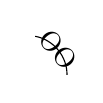
\begin{tikzpicture}[baseline,scale = 0.5]

\tikzset{
point/.style={
thick,
draw,
cross out,
inner sep=0pt,
minimum width=5pt,
minimum height=5pt,
},
}
\clip (0,0) rectangle (1.2,1.2);
\draw[color={black}] (1,0) arc (0:79:1) ;
\draw [color={black}] (0.77,0.64) node[anchor = center,scale=1, rotate = -50.27] {OO};

\end{tikzpicture}\,?\\\textbf {b.} Comment peut-on nommer l'angle marqué par le symbole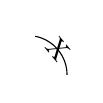
\begin{tikzpicture}[baseline,scale = 0.5]

\tikzset{
point/.style={
thick,
draw,
cross out,
inner sep=0pt,
minimum width=5pt,
minimum height=5pt,
},
}
\clip (0,0) rectangle (1.2,1.2);
\draw[color={black}] (1,0) arc (0:79:1) ;
\draw [color={black}] (0.77,0.64) node[anchor = center,scale=1, rotate = -50.27] {X};

\end{tikzpicture}\,?\\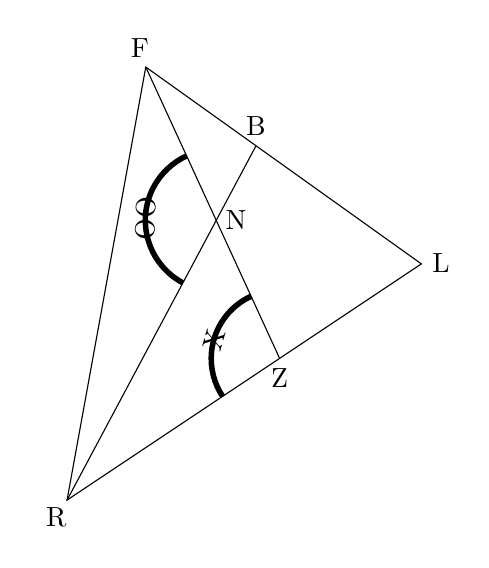
\begin{tikzpicture}[baseline,scale = 0.5]

\tikzset{
point/.style={
thick,
draw,
cross out,
inner sep=0pt,
minimum width=5pt,
minimum height=5pt,
},
}
\clip (-10,-6) rectangle (1,7);
\draw[color={black},line width = 2] (-6.06,0.52) arc (-118.13:-245.36:1.8) ;
\draw [color={black}] (-7.01,2.16) node[anchor = center,scale=1, rotate = 88.41] {OO};
\draw[color={black},line width = 2] (-4.32,0.18) arc (114.5:213.55:1.74) ;
\draw [color={black}] (-5.27,-0.92) node[anchor = center,scale=1, rotate = 73.96000000000001] {X};
\draw[color={black}] (0,1)--(-7,6)--(-9,-5)--cycle;
\draw [color={black}] (0.5,1.03) node[anchor = center,scale=1, rotate = 0] {L};
\draw [color={black}] (-7.15,6.48) node[anchor = center,scale=1, rotate = 0] {F};
\draw [color={black}] (-9.27,-5.42) node[anchor = center,scale=1, rotate = 0] {R};
\draw[color ={black}] (-7,6)--(-3.6,-1.4);
\draw[color ={black}] (-9,-5)--(-4.2,4);
\draw [color={black}] (-4.2,4.5) node[anchor = center,scale=1, rotate = 0] {B};
\draw [color={black}] (-3.6,-1.9) node[anchor = center,scale=1, rotate = 0] {Z};
\draw [color={black}] (-4.71,2.11) node[anchor = center,scale=1, rotate = 0] {N};

\end{tikzpicture}\\ 
\item  \textbf {a.} Comment peut-on nommer l'angle marqué par le symbole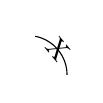
\begin{tikzpicture}[baseline,scale = 0.5]

\tikzset{
point/.style={
thick,
draw,
cross out,
inner sep=0pt,
minimum width=5pt,
minimum height=5pt,
},
}
\clip (0,0) rectangle (1.2,1.2);
\draw[color={black}] (1,0) arc (0:79:1) ;
\draw [color={black}] (0.77,0.64) node[anchor = center,scale=1, rotate = -50.27] {X};

\end{tikzpicture}\,?\\\textbf {b.} Comment peut-on nommer l'angle marqué par le symbole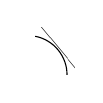
\begin{tikzpicture}[baseline,scale = 0.5]

\tikzset{
point/.style={
thick,
draw,
cross out,
inner sep=0pt,
minimum width=5pt,
minimum height=5pt,
},
}
\clip (0,0) rectangle (1.2,1.2);
\draw[color={black}] (1,0) arc (0:79:1) ;
\draw [color={black}] (0.77,0.64) node[anchor = center,scale=1, rotate = -50.27] {|||};

\end{tikzpicture}\,?\\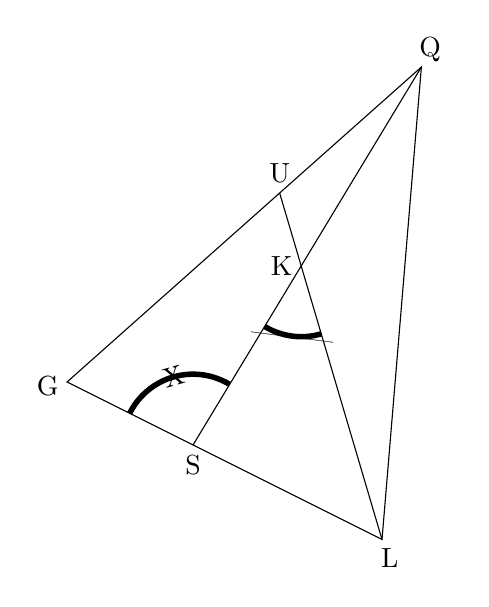
\begin{tikzpicture}[baseline,scale = 0.5]

\tikzset{
point/.style={
thick,
draw,
cross out,
inner sep=0pt,
minimum width=5pt,
minimum height=5pt,
},
}
\clip (-1,-5) rectangle (10,9);
\draw[color={black},line width = 2] (4.13,-0.06) arc (58.87:153.45:1.8) ;
\draw [color={black}] (2.7,0.13) node[anchor = center,scale=1, rotate = 16.120000000000005] {X};
\draw[color={black},line width = 2] (5.02,1.41) arc (-121.13:-73.55:1.8) ;
\draw [color={black}] (5.72,1.17) node[anchor = center,scale=1, rotate = -187.36] {|||};
\draw[color={black}] (0,0)--(9,8)--(8,-4)--cycle;
\draw [color={black}] (-0.49,-0.11) node[anchor = center,scale=1, rotate = 0] {G};
\draw [color={black}] (9.22,8.45) node[anchor = center,scale=1, rotate = 0] {Q};
\draw [color={black}] (8.2,-4.46) node[anchor = center,scale=1, rotate = 0] {L};
\draw[color ={black}] (9,8)--(3.2,-1.6);
\draw[color ={black}] (8,-4)--(5.4,4.8);
\draw [color={black}] (5.4,5.3) node[anchor = center,scale=1, rotate = 0] {U};
\draw [color={black}] (3.2,-2.1) node[anchor = center,scale=1, rotate = 0] {S};
\draw [color={black}] (5.45,2.95) node[anchor = center,scale=1, rotate = 0] {K};

\end{tikzpicture}\\ 
\end{enumerate}
\end{multicols}
\end{exercicedevoir}

\begin{exercicedevoir}[1]
\begin{multicols}{2}
\begin{enumerate}[itemsep=1em]
\item  À propos de l'angle ci-dessous, compléter chaque phrase par la case adéquate.\\\begin{tikzpicture}[baseline,scale = 0.6]

\tikzset{
point/.style={
thick,
draw,
cross out,
inner sep=0pt,
minimum width=5pt,
minimum height=5pt,
},
}
\clip (-6,-2) rectangle (3,5);
\draw[color ={black},line width = 0.625,opacity = 0.8] (-4.19,2.19)--(-3.81,1.81);\draw[color ={black},line width = 0.625,opacity = 0.8] (-4.19,1.81)--(-3.81,2.19);\draw[color ={black},line width = 0.625,opacity = 0.8] (0.81,0.19)--(1.19,-0.19);\draw[color ={black},line width = 0.625,opacity = 0.8] (0.81,-0.19)--(1.19,0.19);\draw[color ={black},line width = 0.625,opacity = 0.8] (0.81,3.19)--(1.19,2.81);\draw[color ={black},line width = 0.625,opacity = 0.8] (0.81,2.81)--(1.19,3.19);
\draw [color={black}] (-3.58,2.84) node[anchor = center,scale=1, rotate = 0] {D};
\draw [color={black}] (0.48,2.95) node[anchor = center,scale=1, rotate = 0] {O};
\draw [color={black}] (2,-0.4) node[anchor = center,scale=1, rotate = 0] {H};
\draw[color={black}] (-0.86,0.74) arc (158.3:90.10000000000001:2) ;
\draw[color ={black}] (1,0)--(-13.28,5.71);
\draw[color ={black}] (1,0)--(1,13);

\end{tikzpicture}\\\\\textbf {a.} $D$ est :\\\\	$\square\;$ le sommet\qquad $\square\;$ un côté\qquad $\square\;$ le nom de l'angle\qquad $\square\;$ rien de cela\qquad 

\medskip
\textbf {b.} $[HO)$ est :\\\\	$\square\;$ le sommet\qquad $\square\;$ un côté\qquad $\square\;$ le nom de l'angle\qquad $\square\;$ rien de cela\qquad 

\medskip
\textbf {c.} $H$ est :\\\\	$\square\;$ le sommet\qquad $\square\;$ un côté\qquad $\square\;$ le nom de l'angle\qquad $\square\;$ rien de cela\qquad 

\medskip
\textbf {d.} $\widehat{DHO}$ est :\\\\	$\square\;$ le sommet\qquad $\square\;$ un côté\qquad $\square\;$ le nom de l'angle\qquad $\square\;$ rien de cela\qquad  
\item  À propos de l'angle ci-dessous, compléter chaque phrase par la case adéquate.\\\begin{tikzpicture}[baseline,scale = 0.6]

\tikzset{
point/.style={
thick,
draw,
cross out,
inner sep=0pt,
minimum width=5pt,
minimum height=5pt,
},
}
\clip (-1,-4) rectangle (6,5);
\draw[color ={black},line width = 0.625,opacity = 0.8] (2.81,-1.81)--(3.19,-2.19);\draw[color ={black},line width = 0.625,opacity = 0.8] (2.81,-2.19)--(3.19,-1.81);\draw[color ={black},line width = 0.625,opacity = 0.8] (3.81,3.19)--(4.19,2.81);\draw[color ={black},line width = 0.625,opacity = 0.8] (3.81,2.81)--(4.19,3.19);\draw[color ={black},line width = 0.625,opacity = 0.8] (0.81,3.19)--(1.19,2.81);\draw[color ={black},line width = 0.625,opacity = 0.8] (0.81,2.81)--(1.19,3.19);
\draw [color={black}] (2.15,-1.75) node[anchor = center,scale=1, rotate = 0] {U};
\draw [color={black}] (1.05,2.48) node[anchor = center,scale=1, rotate = 0] {J};
\draw [color={black}] (4.2,4) node[anchor = center,scale=1, rotate = 0] {L};
\draw[color={black}] (3.61,1.04) arc (-101.25:-179.94:2) ;
\draw[color ={black}] (4,3)--(1.04,-11.8);
\draw[color ={black}] (4,3)--(-9,3);

\end{tikzpicture}\\\\\textbf {a.} $U$ est :\\\\	$\square\;$ le sommet\qquad $\square\;$ un côté\qquad $\square\;$ le nom de l'angle\qquad $\square\;$ rien de cela\qquad 

\medskip
\textbf {b.} $[LJ)$ est :\\\\	$\square\;$ le sommet\qquad $\square\;$ un côté\qquad $\square\;$ le nom de l'angle\qquad $\square\;$ rien de cela\qquad 

\medskip
\textbf {c.} $L$ est :\\\\	$\square\;$ le sommet\qquad $\square\;$ un côté\qquad $\square\;$ le nom de l'angle\qquad $\square\;$ rien de cela\qquad 

\medskip
\textbf {d.} $\widehat{ULJ}$ est :\\\\	$\square\;$ le sommet\qquad $\square\;$ un côté\qquad $\square\;$ le nom de l'angle\qquad $\square\;$ rien de cela\qquad  
\end{enumerate}
\end{multicols}
\end{exercicedevoir}

\begin{exercicedevoir}[1]
\begin{multicols}{2}
\begin{enumerate}[itemsep=1em]
\item  Dans la figure ci-dessous :\\\begin{tikzpicture}[baseline,scale = 0.4]

\tikzset{
point/.style={
thick,
draw,
cross out,
inner sep=0pt,
minimum width=5pt,
minimum height=5pt,
},
}
\clip (-6.24,-2.2) rectangle (2.2,5.07);
\draw[color ={black},line width = 0.625,opacity = 0.8] (-0.19,0.19)--(0.19,-0.19);\draw[color ={black},line width = 0.625,opacity = 0.8] (-0.19,-0.19)--(0.19,0.19);\draw[color ={black},line width = 0.625,opacity = 0.8] (-1.07,3.06)--(-0.69,2.68);\draw[color ={black},line width = 0.625,opacity = 0.8] (-1.07,2.68)--(-0.69,3.06);\draw[color ={black},line width = 0.625,opacity = 0.8] (-4.23,0.6)--(-3.85,0.22);\draw[color ={black},line width = 0.625,opacity = 0.8] (-4.23,0.22)--(-3.85,0.6);
\draw [color={black}] (0.49,0.2) node[anchor = center,scale=1, rotate = 0] {R};
\draw [color={black}] (-4.42,1) node[anchor = center,scale=1, rotate = 0] {J};
\draw [color={black}] (-0.37,2.98) node[anchor = center,scale=1, rotate = 0] {U};
\draw[color={black}] (-0.29,0.96) arc (-72.83:-141.98000000000002:2) ;
\draw[color ={black}] (-0.88,2.87)--(2.93,-9.57);
\draw[color ={black}] (-0.88,2.87)--(-11.94,-5.74);

\end{tikzpicture}\\\\$\widehat{RUJ}$ est un angle :\\\\	$\square\;$ nul\qquad $\square\;$ aigu\qquad $\square\;$ droit\qquad $\square\;$ obtus\qquad $\square\;$ plat\qquad  
\item  Dans la figure ci-dessous :\\\begin{tikzpicture}[baseline,scale = 0.4]

\tikzset{
point/.style={
thick,
draw,
cross out,
inner sep=0pt,
minimum width=5pt,
minimum height=5pt,
},
}
\clip (-2.2,-2.2) rectangle (8.29,4.67);
\draw[color ={black},line width = 0.625,opacity = 0.8] (-0.19,0.19)--(0.19,-0.19);\draw[color ={black},line width = 0.625,opacity = 0.8] (-0.19,-0.19)--(0.19,0.19);\draw[color ={black},line width = 0.625,opacity = 0.8] (2.63,0.35)--(3.01,-0.03);\draw[color ={black},line width = 0.625,opacity = 0.8] (2.63,-0.03)--(3.01,0.35);\draw[color ={black},line width = 0.625,opacity = 0.8] (5.9,2.66)--(6.28,2.28);\draw[color ={black},line width = 0.625,opacity = 0.8] (5.9,2.28)--(6.28,2.66);
\draw [color={black}] (0.07,-0.49) node[anchor = center,scale=1, rotate = 0] {I};
\draw [color={black}] (6.44,1.87) node[anchor = center,scale=1, rotate = 0] {V};
\draw [color={black}] (2.8,-0.33) node[anchor = center,scale=1, rotate = 0] {D};
\draw[color={black}] (0.82,0.05) arc (-176.85:-324.86:2) ;
\draw[color ={black}] (2.82,0.16)--(-10,-0.57);
\draw[color ={black}] (2.82,0.16)--(14.27,8.25);

\end{tikzpicture}\\\\$\widehat{IDV}$ est un angle :\\\\	$\square\;$ nul\qquad $\square\;$ aigu\qquad $\square\;$ droit\qquad $\square\;$ obtus\qquad $\square\;$ plat\qquad  
\item  Dans la figure ci-dessous :\\\begin{tikzpicture}[baseline,scale = 0.4]

\tikzset{
point/.style={
thick,
draw,
cross out,
inner sep=0pt,
minimum width=5pt,
minimum height=5pt,
},
}
\clip (-2.2,-4.970000000000001) rectangle (8.780000000000001,2.2);
\draw[color ={black},line width = 0.625,opacity = 0.8] (-0.19,0.19)--(0.19,-0.19);\draw[color ={black},line width = 0.625,opacity = 0.8] (-0.19,-0.19)--(0.19,0.19);\draw[color ={black},line width = 0.625,opacity = 0.8] (2.71,-1.03)--(3.09,-1.41);\draw[color ={black},line width = 0.625,opacity = 0.8] (2.71,-1.41)--(3.09,-1.03);\draw[color ={black},line width = 0.625,opacity = 0.8] (6.39,-2.58)--(6.77,-2.96);\draw[color ={black},line width = 0.625,opacity = 0.8] (6.39,-2.96)--(6.77,-2.58);
\draw [color={black}] (-0.17,-0.52) node[anchor = center,scale=1, rotate = 0] {O};
\draw [color={black}] (6.25,-3.39) node[anchor = center,scale=1, rotate = 0] {H};
\draw [color={black}] (2.64,-1.71) node[anchor = center,scale=1, rotate = 0] {D};
\draw[color={black}] (1.06,-0.45) arc (157.29:337.27:1.99) ;
\draw[color ={black}] (2.9,-1.22)--(-9.21,3.87);
\draw[color ={black}] (2.9,-1.22)--(15.8,-6.65);

\end{tikzpicture}\\\\$\widehat{ODH}$ est un angle :\\\\	$\square\;$ nul\qquad $\square\;$ aigu\qquad $\square\;$ droit\qquad $\square\;$ obtus\qquad $\square\;$ plat\qquad  
\item  Dans la figure ci-dessous :\\\begin{tikzpicture}[baseline,scale = 0.4]

\tikzset{
point/.style={
thick,
draw,
cross out,
inner sep=0pt,
minimum width=5pt,
minimum height=5pt,
},
}
\clip (-5.2,-6.3) rectangle (2.2,2.2);
\draw[color ={black},line width = 0.625,opacity = 0.8] (-0.19,0.19)--(0.19,-0.19);\draw[color ={black},line width = 0.625,opacity = 0.8] (-0.19,-0.19)--(0.19,0.19);\draw[color ={black},line width = 0.625,opacity = 0.8] (-3.19,0.09)--(-2.81,-0.29);\draw[color ={black},line width = 0.625,opacity = 0.8] (-3.19,-0.29)--(-2.81,0.09);\draw[color ={black},line width = 0.625,opacity = 0.8] (-3.06,-3.91)--(-2.68,-4.29);\draw[color ={black},line width = 0.625,opacity = 0.8] (-3.06,-4.29)--(-2.68,-3.91);
\draw [color={black}] (-0.06,0.52) node[anchor = center,scale=1, rotate = 0] {Z};
\draw [color={black}] (-3.57,-4.06) node[anchor = center,scale=1, rotate = 0] {O};
\draw [color={black}] (-2.97,0.42) node[anchor = center,scale=1, rotate = 0] {G};
\draw[color={black}] (-2,-0.07) arc (1.72:-88.33:1) ;
\draw[color ={black}] (-3,-0.1)--(10,0.33);
\draw[color ={black}] (-3,-0.1)--(-2.55,-14.1);

\end{tikzpicture}\\\\$\widehat{ZGO}$ est un angle :\\\\	$\square\;$ nul\qquad $\square\;$ aigu\qquad $\square\;$ droit\qquad $\square\;$ obtus\qquad $\square\;$ plat\qquad  
\end{enumerate}
\end{multicols}
\end{exercicedevoir}

\begin{exercicedevoir}[1]


\begin{multicols}{2}
\begin{enumerate}[itemsep=1em]
\item  Estimer la mesure de l'angle $\widehat{xGw}$ sans instrument.\\\begin{tikzpicture}[baseline,scale = 0.7]

\tikzset{
point/.style={
thick,
draw,
cross out,
inner sep=0pt,
minimum width=5pt,
minimum height=5pt,
},
}
\clip (-1,-2.55) rectangle (6.98,1);
\draw[color ={black}] (0,0)--(15.47,-4.13);
\draw[color ={black}] (0,0)--(15.95,-1.39);
\draw [color={black}] (-0.49,0.09) node[anchor = center,scale=1.5, rotate = 0] {G};
\draw [color={black}] (5.36,-2.02) node[anchor = center,scale=1.5, rotate = 0] {x};
\draw [color={black}] (5.73,0.08) node[anchor = center,scale=1.5, rotate = 0] {w};
\draw (1.97,-0.35) node[anchor = center] {\footnotesize \color{black}{$ $}};
\draw[color={black}] (1.45,-0.39) arc (-15.05:-5.0600000000000005:1.5) ;

\end{tikzpicture}\\\\\\	$\square\;$ $145^\circ$\qquad $\square\;$ $100^\circ$\qquad $\square\;$ $90^\circ$\qquad $\square\;$ $10^\circ$\qquad $\square\;$ $55^\circ$\qquad $\square\;$ $180^\circ$\qquad  
\item  Estimer la mesure de l'angle $\widehat{tCv}$ sans instrument.\\\begin{tikzpicture}[baseline,scale = 0.7]

\tikzset{
point/.style={
thick,
draw,
cross out,
inner sep=0pt,
minimum width=5pt,
minimum height=5pt,
},
}
\clip (-2.56,-6.8) rectangle (6.98,1.52);
\draw[color ={black}] (0,0)--(15.95,1.39);
\draw[color ={black}] (0,0)--(-4.16,-15.45);
\draw [color={black}] (-0.32,0.38) node[anchor = center,scale=1.5, rotate = 0] {C};
\draw [color={black}] (5.63,1.06) node[anchor = center,scale=1.5, rotate = 0] {t};
\draw [color={black}] (-2.03,-5.36) node[anchor = center,scale=1.5, rotate = 0] {v};
\draw (1.28,-1.53) node[anchor = center] {\footnotesize \color{black}{$ $}};
\draw[color={black}] (1.5,0.13) arc (4.95:-105.07:1.51) ;

\end{tikzpicture}\\\\\\	$\square\;$ $155^\circ$\qquad $\square\;$ $20^\circ$\qquad $\square\;$ $90^\circ$\qquad $\square\;$ $110^\circ$\qquad $\square\;$ $180^\circ$\qquad $\square\;$ $65^\circ$\qquad  
\item  Estimer la mesure de l'angle $\widehat{xFu}$ sans instrument.\\\begin{tikzpicture}[baseline,scale = 0.7]

\tikzset{
point/.style={
thick,
draw,
cross out,
inner sep=0pt,
minimum width=5pt,
minimum height=5pt,
},
}
\clip (-1,-6.64) rectangle (6.91,2.04);
\draw[color ={black}] (0,0)--(15.76,2.77);
\draw[color ={black}] (0,0)--(5.47,-15.04);
\draw [color={black}] (-0.43,0.25) node[anchor = center,scale=1.5, rotate = 0] {F};
\draw [color={black}] (5.51,1.55) node[anchor = center,scale=1.5, rotate = 0] {x};
\draw [color={black}] (1.41,-5.56) node[anchor = center,scale=1.5, rotate = 0] {u};
\draw (1.73,-1) node[anchor = center] {\footnotesize \color{black}{$ $}};
\draw[color={black}] (1.48,0.26) arc (9.96:-70.05000000000001:1.5) ;

\end{tikzpicture}\\\\\\	$\square\;$ $180^\circ$\qquad $\square\;$ $170^\circ$\qquad $\square\;$ $90^\circ$\qquad $\square\;$ $80^\circ$\qquad $\square\;$ $35^\circ$\qquad $\square\;$ $125^\circ$\qquad  
\item  Estimer la mesure de l'angle $\widehat{tIu}$ sans instrument.\\\begin{tikzpicture}[baseline,scale = 0.7]

\tikzset{
point/.style={
thick,
draw,
cross out,
inner sep=0pt,
minimum width=5pt,
minimum height=5pt,
},
}
\clip (-1,-2.04) rectangle (6.91,7);
\draw[color ={black}] (0,0)--(15.76,-2.77);
\draw[color ={black}] (0,0)--(0,16);
\draw [color={black}] (-0.38,-0.32) node[anchor = center,scale=1.5, rotate = 0] {I};
\draw [color={black}] (5.51,-1.55) node[anchor = center,scale=1.5, rotate = 0] {t};
\draw [color={black}] (-0.57,5.7) node[anchor = center,scale=1.5, rotate = 0] {u};
\draw (1.53,1.28) node[anchor = center] {\footnotesize \color{black}{$ $}};
\draw[color={black}] (1.48,-0.26) arc (-9.96:90.02000000000001:1.5) ;

\end{tikzpicture}\\\\\\	$\square\;$ $55^\circ$\qquad $\square\;$ $10^\circ$\qquad $\square\;$ $90^\circ$\qquad $\square\;$ $180^\circ$\qquad $\square\;$ $145^\circ$\qquad $\square\;$ $100^\circ$\qquad  
\end{enumerate}
\end{multicols}
\end{exercicedevoir}

\begin{exercicedevoir}[1]

\begin{enumerate}[itemsep=1em]
\item \textbf {a.}  Quelle est la mesure, en degrés, de l'angle $\widehat{VGM}$ ?\\\textbf {b.}  Quelle est la mesure, en degrés, de l'angle $\widehat{MGC}$ ?\\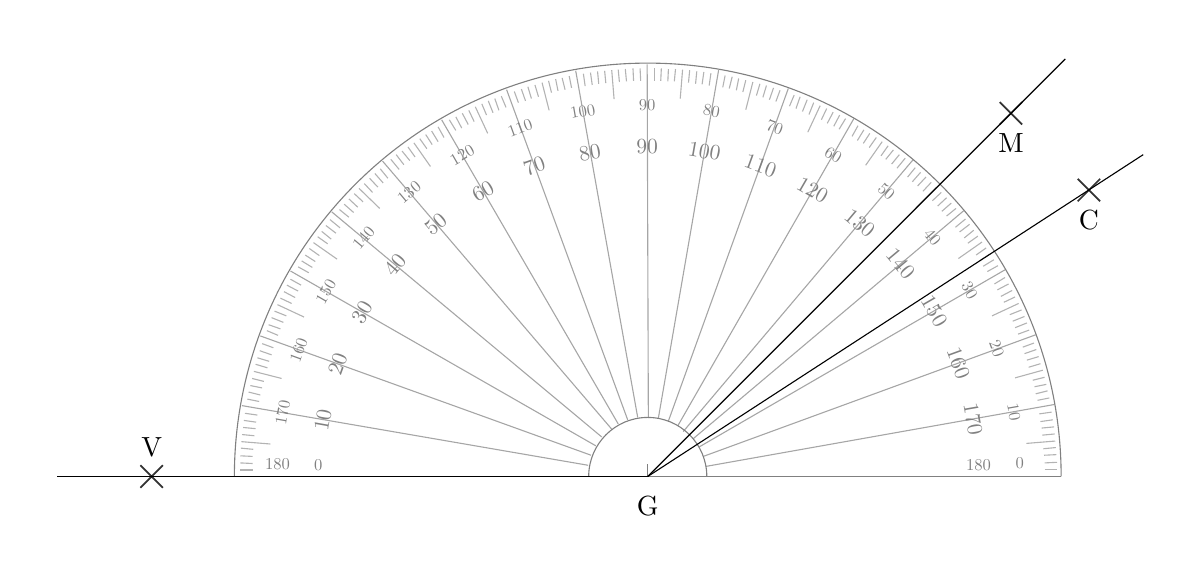
\begin{tikzpicture}[baseline,scale = 0.75]

\tikzset{
point/.style={
thick,
draw,
cross out,
inner sep=0pt,
minimum width=5pt,
minimum height=5pt,
},
}
\clip (-10.5,-1.3) rectangle (8.89,7.6);
\draw[color ={gray}] (7,0)--(-7,0);
\draw[color={gray}] (1,0) arc (0:179.9:1) ;
\draw[color={gray}] (7,0) arc (0:179.9:7) ;
\draw [color={gray}] (5.6,0.2) node[anchor = center,scale=0.6, rotate = 360] {180};
\draw [color={gray}] (5.51,0.97) node[anchor = center,scale=0.78, rotate = 280] {170};
\draw [color={gray}] (6.3,0.22) node[anchor = center,scale=0.6, rotate = 360] {0};
\draw [color={gray}] (6.2,1.09) node[anchor = center,scale=0.6, rotate = 280] {10};
\draw[color ={gray},opacity = 0.6] (6.72,0.12)--(6.93,0.12);
\draw[color ={gray},opacity = 0.6] (6.72,0.23)--(6.93,0.24);
\draw[color ={gray},opacity = 0.6] (6.71,0.36)--(6.92,0.37);
\draw[color ={gray},opacity = 0.6] (6.7,0.47)--(6.91,0.49);
\draw[color ={gray},opacity = 0.6] (6.41,0.56)--(6.9,0.6);
\draw[color ={gray},opacity = 0.6] (6.68,0.7)--(6.89,0.72);
\draw[color ={gray},opacity = 0.6] (6.67,0.82)--(6.88,0.84);
\draw[color ={gray},opacity = 0.6] (6.65,0.93)--(6.86,0.96);
\draw[color ={gray},opacity = 0.6] (6.63,1.06)--(6.84,1.09);
\draw [color={gray}] (5.26,1.92) node[anchor = center,scale=0.78, rotate = 290] {160};
\draw [color={gray}] (5.91,2.16) node[anchor = center,scale=0.6, rotate = 290] {20};
\draw[color ={gray},opacity = 0.6] (6.6,1.29)--(6.8,1.33);
\draw[color ={gray},opacity = 0.6] (6.57,1.4)--(6.77,1.45);
\draw[color ={gray},opacity = 0.6] (6.55,1.52)--(6.75,1.56);
\draw[color ={gray},opacity = 0.6] (6.52,1.63)--(6.72,1.68);
\draw[color ={gray},opacity = 0.6] (6.22,1.67)--(6.69,1.8);
\draw[color ={gray},opacity = 0.6] (6.45,1.85)--(6.65,1.91);
\draw[color ={gray},opacity = 0.6] (6.42,1.97)--(6.62,2.03);
\draw[color ={gray},opacity = 0.6] (6.38,2.08)--(6.58,2.15);
\draw[color ={gray},opacity = 0.6] (6.35,2.19)--(6.54,2.26);
\draw[color ={gray},opacity = 0.7] (0.98,0.17)--(6.89,1.22);
\draw [color={gray}] (4.85,2.8) node[anchor = center,scale=0.78, rotate = 300] {150};
\draw [color={gray}] (5.45,3.15) node[anchor = center,scale=0.6, rotate = 300] {30};
\draw[color ={gray},opacity = 0.6] (6.27,2.41)--(6.46,2.48);
\draw[color ={gray},opacity = 0.6] (6.22,2.52)--(6.42,2.6);
\draw[color ={gray},opacity = 0.6] (6.18,2.63)--(6.38,2.71);
\draw[color ={gray},opacity = 0.6] (6.13,2.74)--(6.33,2.82);
\draw[color ={gray},opacity = 0.6] (5.83,2.72)--(6.28,2.93);
\draw[color ={gray},opacity = 0.6] (6.03,2.95)--(6.22,3.04);
\draw[color ={gray},opacity = 0.6] (5.98,3.05)--(6.17,3.15);
\draw[color ={gray},opacity = 0.6] (5.92,3.16)--(6.11,3.26);
\draw[color ={gray},opacity = 0.6] (5.87,3.26)--(6.05,3.37);
\draw[color ={gray},opacity = 0.7] (0.94,0.34)--(6.57,2.4);
\draw [color={gray}] (4.28,3.6) node[anchor = center,scale=0.78, rotate = 310] {140};
\draw [color={gray}] (4.82,4.05) node[anchor = center,scale=0.6, rotate = 310] {40};
\draw[color ={gray},opacity = 0.6] (5.75,3.47)--(5.93,3.57);
\draw[color ={gray},opacity = 0.6] (5.68,3.56)--(5.86,3.67);
\draw[color ={gray},opacity = 0.6] (5.63,3.66)--(5.8,3.77);
\draw[color ={gray},opacity = 0.6] (5.56,3.75)--(5.73,3.87);
\draw[color ={gray},opacity = 0.6] (5.26,3.69)--(5.66,3.97);
\draw[color ={gray},opacity = 0.6] (5.42,3.95)--(5.59,4.07);
\draw[color ={gray},opacity = 0.6] (5.36,4.04)--(5.52,4.17);
\draw[color ={gray},opacity = 0.6] (5.28,4.14)--(5.45,4.27);
\draw[color ={gray},opacity = 0.6] (5.21,4.22)--(5.38,4.36);
\draw[color ={gray},opacity = 0.7] (0.87,0.5)--(6.05,3.5);
\draw [color={gray}] (3.59,4.29) node[anchor = center,scale=0.78, rotate = 320] {130};
\draw [color={gray}] (4.04,4.83) node[anchor = center,scale=0.6, rotate = 320] {50};
\draw[color ={gray},opacity = 0.6] (5.06,4.41)--(5.22,4.54);
\draw[color ={gray},opacity = 0.6] (4.98,4.49)--(5.14,4.63);
\draw[color ={gray},opacity = 0.6] (4.91,4.58)--(5.06,4.72);
\draw[color ={gray},opacity = 0.6] (4.82,4.67)--(4.97,4.81);
\draw[color ={gray},opacity = 0.6] (4.54,4.55)--(4.89,4.9);
\draw[color ={gray},opacity = 0.6] (4.66,4.83)--(4.8,4.98);
\draw[color ={gray},opacity = 0.6] (4.57,4.92)--(4.71,5.07);
\draw[color ={gray},opacity = 0.6] (4.48,4.99)--(4.62,5.15);
\draw[color ={gray},opacity = 0.6] (4.4,5.07)--(4.53,5.23);
\draw[color ={gray},opacity = 0.7] (0.77,0.64)--(5.35,4.5);
\draw [color={gray}] (2.79,4.85) node[anchor = center,scale=0.78, rotate = 330] {120};
\draw [color={gray}] (3.14,5.45) node[anchor = center,scale=0.6, rotate = 330] {60};
\draw[color ={gray},opacity = 0.6] (4.22,5.22)--(4.36,5.39);
\draw[color ={gray},opacity = 0.6] (4.13,5.29)--(4.26,5.45);
\draw[color ={gray},opacity = 0.6] (4.03,5.37)--(4.16,5.53);
\draw[color ={gray},opacity = 0.6] (3.95,5.43)--(4.07,5.6);
\draw[color ={gray},opacity = 0.6] (3.69,5.27)--(3.97,5.67);
\draw[color ={gray},opacity = 0.6] (3.75,5.57)--(3.87,5.74);
\draw[color ={gray},opacity = 0.6] (3.65,5.64)--(3.76,5.81);
\draw[color ={gray},opacity = 0.6] (3.55,5.69)--(3.66,5.87);
\draw[color ={gray},opacity = 0.6] (3.46,5.76)--(3.56,5.94);
\draw[color ={gray},opacity = 0.7] (0.6,0.76)--(4.49,5.36);
\draw [color={gray}] (1.91,5.26) node[anchor = center,scale=0.78, rotate = 340] {110};
\draw [color={gray}] (2.15,5.91) node[anchor = center,scale=0.6, rotate = 340] {70};
\draw[color ={gray},opacity = 0.6] (3.24,5.88)--(3.35,6.06);
\draw[color ={gray},opacity = 0.6] (3.15,5.93)--(3.25,6.12);
\draw[color ={gray},opacity = 0.6] (3.04,5.98)--(3.14,6.17);
\draw[color ={gray},opacity = 0.6] (2.94,6.04)--(3.03,6.23);
\draw[color ={gray},opacity = 0.6] (2.71,5.83)--(2.92,6.28);
\draw[color ={gray},opacity = 0.6] (2.73,6.13)--(2.81,6.33);
\draw[color ={gray},opacity = 0.6] (2.62,6.18)--(2.7,6.38);
\draw[color ={gray},opacity = 0.6] (2.51,6.23)--(2.58,6.43);
\draw[color ={gray},opacity = 0.6] (2.4,6.27)--(2.48,6.46);
\draw[color ={gray},opacity = 0.7] (0.51,0.86)--(3.49,6.06);
\draw [color={gray}] (0.96,5.51) node[anchor = center,scale=0.78, rotate = 350] {100};
\draw [color={gray}] (1.08,6.19) node[anchor = center,scale=0.6, rotate = 350] {80};
\draw[color ={gray},opacity = 0.6] (2.17,6.35)--(2.24,6.54);
\draw[color ={gray},opacity = 0.6] (2.06,6.38)--(2.13,6.58);
\draw[color ={gray},opacity = 0.6] (1.95,6.42)--(2.01,6.62);
\draw[color ={gray},opacity = 0.6] (1.84,6.45)--(1.9,6.65);
\draw[color ={gray},opacity = 0.6] (1.66,6.21)--(1.78,6.68);
\draw[color ={gray},opacity = 0.6] (1.61,6.51)--(1.66,6.71);
\draw[color ={gray},opacity = 0.6] (1.5,6.54)--(1.54,6.74);
\draw[color ={gray},opacity = 0.6] (1.38,6.57)--(1.43,6.77);
\draw[color ={gray},opacity = 0.6] (1.27,6.59)--(1.31,6.79);
\draw[color ={gray},opacity = 0.7] (0.35,0.94)--(2.38,6.57);
\draw [color={gray}] (-0.01,5.58) node[anchor = center,scale=0.78, rotate = 360] {90};
\draw [color={gray}] (-0.01,6.28) node[anchor = center,scale=0.6, rotate = 360] {90};
\draw[color ={gray},opacity = 0.6] (1.04,6.62)--(1.07,6.83);
\draw[color ={gray},opacity = 0.6] (0.92,6.64)--(0.95,6.85);
\draw[color ={gray},opacity = 0.6] (0.81,6.65)--(0.83,6.86);
\draw[color ={gray},opacity = 0.6] (0.69,6.67)--(0.71,6.88);
\draw[color ={gray},opacity = 0.6] (0.55,6.4)--(0.59,6.89);
\draw[color ={gray},opacity = 0.6] (0.45,6.69)--(0.47,6.9);
\draw[color ={gray},opacity = 0.6] (0.34,6.69)--(0.35,6.9);
\draw[color ={gray},opacity = 0.6] (0.22,6.7)--(0.23,6.91);
\draw[color ={gray},opacity = 0.6] (0.11,6.7)--(0.11,6.91);
\draw[color ={gray},opacity = 0.7] (0.18,0.99)--(1.2,6.88);
\draw [color={gray}] (-0.98,5.49) node[anchor = center,scale=0.78, rotate = 370] {80};
\draw [color={gray}] (-1.1,6.18) node[anchor = center,scale=0.6, rotate = 370] {100};
\draw[color ={gray},opacity = 0.6] (-0.12,6.7)--(-0.13,6.91);
\draw[color ={gray},opacity = 0.6] (-0.24,6.7)--(-0.25,6.91);
\draw[color ={gray},opacity = 0.6] (-0.36,6.69)--(-0.38,6.9);
\draw[color ={gray},opacity = 0.6] (-0.48,6.68)--(-0.5,6.89);
\draw[color ={gray},opacity = 0.6] (-0.57,6.39)--(-0.61,6.88);
\draw[color ={gray},opacity = 0.6] (-0.71,6.66)--(-0.73,6.87);
\draw[color ={gray},opacity = 0.6] (-0.83,6.65)--(-0.85,6.86);
\draw[color ={gray},opacity = 0.6] (-0.94,6.63)--(-0.97,6.84);
\draw[color ={gray},opacity = 0.6] (-1.06,6.61)--(-1.09,6.82);
\draw[color ={gray},opacity = 0.7] (0.01,1.01)--(-0.01,6.98);
\draw [color={gray}] (-1.92,5.25) node[anchor = center,scale=0.78, rotate = 380] {70};
\draw [color={gray}] (-2.16,5.9) node[anchor = center,scale=0.6, rotate = 380] {110};
\draw[color ={gray},opacity = 0.6] (-1.29,6.58)--(-1.33,6.78);
\draw[color ={gray},opacity = 0.6] (-1.4,6.55)--(-1.45,6.75);
\draw[color ={gray},opacity = 0.6] (-1.52,6.53)--(-1.56,6.73);
\draw[color ={gray},opacity = 0.6] (-1.63,6.5)--(-1.68,6.7);
\draw[color ={gray},opacity = 0.6] (-1.67,6.2)--(-1.79,6.67);
\draw[color ={gray},opacity = 0.6] (-1.85,6.43)--(-1.91,6.63);
\draw[color ={gray},opacity = 0.6] (-1.97,6.4)--(-2.03,6.6);
\draw[color ={gray},opacity = 0.6] (-2.07,6.36)--(-2.14,6.56);
\draw[color ={gray},opacity = 0.6] (-2.19,6.33)--(-2.26,6.52);
\draw[color ={gray},opacity = 0.7] (-0.17,1)--(-1.22,6.87);
\draw [color={gray}] (-2.79,4.83) node[anchor = center,scale=0.78, rotate = 390] {60};
\draw [color={gray}] (-3.14,5.44) node[anchor = center,scale=0.6, rotate = 390] {120};
\draw[color ={gray},opacity = 0.6] (-2.4,6.25)--(-2.48,6.44);
\draw[color ={gray},opacity = 0.6] (-2.52,6.2)--(-2.59,6.4);
\draw[color ={gray},opacity = 0.6] (-2.62,6.16)--(-2.7,6.36);
\draw[color ={gray},opacity = 0.6] (-2.73,6.12)--(-2.81,6.31);
\draw[color ={gray},opacity = 0.6] (-2.71,5.81)--(-2.92,6.26);
\draw[color ={gray},opacity = 0.6] (-2.94,6.01)--(-3.03,6.2);
\draw[color ={gray},opacity = 0.6] (-3.04,5.96)--(-3.14,6.15);
\draw[color ={gray},opacity = 0.6] (-3.15,5.9)--(-3.25,6.09);
\draw[color ={gray},opacity = 0.6] (-3.25,5.86)--(-3.36,6.04);
\draw[color ={gray},opacity = 0.7] (-0.34,0.96)--(-2.39,6.55);
\draw [color={gray}] (-3.59,4.27) node[anchor = center,scale=0.78, rotate = 400] {50};
\draw [color={gray}] (-4.04,4.81) node[anchor = center,scale=0.6, rotate = 400] {130};
\draw[color ={gray},opacity = 0.6] (-3.45,5.74)--(-3.55,5.92);
\draw[color ={gray},opacity = 0.6] (-3.55,5.67)--(-3.66,5.85);
\draw[color ={gray},opacity = 0.6] (-3.65,5.62)--(-3.76,5.79);
\draw[color ={gray},opacity = 0.6] (-3.74,5.55)--(-3.86,5.72);
\draw[color ={gray},opacity = 0.6] (-3.68,5.25)--(-3.96,5.65);
\draw[color ={gray},opacity = 0.6] (-3.94,5.41)--(-4.06,5.58);
\draw[color ={gray},opacity = 0.6] (-4.03,5.35)--(-4.16,5.51);
\draw[color ={gray},opacity = 0.6] (-4.13,5.28)--(-4.26,5.45);
\draw[color ={gray},opacity = 0.6] (-4.21,5.2)--(-4.35,5.37);
\draw[color ={gray},opacity = 0.7] (-0.5,0.89)--(-3.49,6.04);
\draw [color={gray}] (-4.28,3.58) node[anchor = center,scale=0.78, rotate = 410] {40};
\draw [color={gray}] (-4.81,4.04) node[anchor = center,scale=0.6, rotate = 410] {140};
\draw[color ={gray},opacity = 0.6] (-4.4,5.05)--(-4.53,5.21);
\draw[color ={gray},opacity = 0.6] (-4.48,4.97)--(-4.62,5.13);
\draw[color ={gray},opacity = 0.6] (-4.57,4.9)--(-4.71,5.05);
\draw[color ={gray},opacity = 0.6] (-4.66,4.81)--(-4.8,4.96);
\draw[color ={gray},opacity = 0.6] (-4.54,4.54)--(-4.89,4.88);
\draw[color ={gray},opacity = 0.6] (-4.82,4.65)--(-4.97,4.79);
\draw[color ={gray},opacity = 0.6] (-4.91,4.56)--(-5.06,4.7);
\draw[color ={gray},opacity = 0.6] (-4.98,4.47)--(-5.14,4.61);
\draw[color ={gray},opacity = 0.6] (-5.06,4.39)--(-5.22,4.52);
\draw[color ={gray},opacity = 0.7] (-0.6,0.79)--(-4.49,5.34);
\draw [color={gray}] (-4.84,2.78) node[anchor = center,scale=0.78, rotate = 420] {30};
\draw [color={gray}] (-5.45,3.13) node[anchor = center,scale=0.6, rotate = 420] {150};
\draw[color ={gray},opacity = 0.6] (-5.21,4.21)--(-5.38,4.35);
\draw[color ={gray},opacity = 0.6] (-5.28,4.12)--(-5.45,4.25);
\draw[color ={gray},opacity = 0.6] (-5.36,4.02)--(-5.52,4.15);
\draw[color ={gray},opacity = 0.6] (-5.42,3.94)--(-5.59,4.06);
\draw[color ={gray},opacity = 0.6] (-5.26,3.68)--(-5.66,3.96);
\draw[color ={gray},opacity = 0.6] (-5.56,3.74)--(-5.73,3.86);
\draw[color ={gray},opacity = 0.6] (-5.63,3.64)--(-5.8,3.75);
\draw[color ={gray},opacity = 0.6] (-5.68,3.54)--(-5.86,3.65);
\draw[color ={gray},opacity = 0.6] (-5.74,3.45)--(-5.92,3.55);
\draw[color ={gray},opacity = 0.7] (-0.78,0.67)--(-5.35,4.48);
\draw [color={gray}] (-5.25,1.9) node[anchor = center,scale=0.78, rotate = 430] {20};
\draw [color={gray}] (-5.91,2.14) node[anchor = center,scale=0.6, rotate = 430] {160};
\draw[color ={gray},opacity = 0.6] (-5.87,3.24)--(-6.05,3.34);
\draw[color ={gray},opacity = 0.6] (-5.92,3.14)--(-6.11,3.24);
\draw[color ={gray},opacity = 0.6] (-5.97,3.03)--(-6.16,3.13);
\draw[color ={gray},opacity = 0.6] (-6.03,2.93)--(-6.22,3.02);
\draw[color ={gray},opacity = 0.6] (-5.82,2.7)--(-6.27,2.91);
\draw[color ={gray},opacity = 0.6] (-6.12,2.72)--(-6.32,2.8);
\draw[color ={gray},opacity = 0.6] (-6.17,2.61)--(-6.37,2.69);
\draw[color ={gray},opacity = 0.6] (-6.22,2.5)--(-6.42,2.57);
\draw[color ={gray},opacity = 0.6] (-6.26,2.39)--(-6.45,2.47);
\draw[color ={gray},opacity = 0.7] (-0.88,0.52)--(-6.05,3.48);
\draw [color={gray}] (-5.5,0.96) node[anchor = center,scale=0.78, rotate = 440] {10};
\draw [color={gray}] (-6.18,1.08) node[anchor = center,scale=0.6, rotate = 440] {170};
\draw[color ={gray},opacity = 0.6] (-6.34,2.18)--(-6.53,2.25);
\draw[color ={gray},opacity = 0.6] (-6.37,2.06)--(-6.57,2.13);
\draw[color ={gray},opacity = 0.6] (-6.41,1.95)--(-6.61,2.01);
\draw[color ={gray},opacity = 0.6] (-6.44,1.84)--(-6.64,1.9);
\draw[color ={gray},opacity = 0.6] (-6.2,1.66)--(-6.67,1.78);
\draw[color ={gray},opacity = 0.6] (-6.5,1.61)--(-6.7,1.66);
\draw[color ={gray},opacity = 0.6] (-6.53,1.5)--(-6.73,1.54);
\draw[color ={gray},opacity = 0.6] (-6.56,1.38)--(-6.76,1.43);
\draw[color ={gray},opacity = 0.6] (-6.58,1.27)--(-6.78,1.31);
\draw[color ={gray},opacity = 0.7] (-0.96,0.36)--(-6.56,2.38);
\draw [color={gray}] (-5.58,0.19) node[anchor = center,scale=0.6, rotate = 360] {0};
\draw [color={gray}] (-6.27,0.21) node[anchor = center,scale=0.6, rotate = 360] {180};
\draw[color ={gray},opacity = 0.6] (-6.61,1.04)--(-6.82,1.07);
\draw[color ={gray},opacity = 0.6] (-6.63,0.92)--(-6.84,0.95);
\draw[color ={gray},opacity = 0.6] (-6.64,0.81)--(-6.85,0.83);
\draw[color ={gray},opacity = 0.6] (-6.66,0.69)--(-6.87,0.71);
\draw[color ={gray},opacity = 0.6] (-6.39,0.55)--(-6.88,0.59);
\draw[color ={gray},opacity = 0.6] (-6.68,0.46)--(-6.89,0.48);
\draw[color ={gray},opacity = 0.6] (-6.69,0.34)--(-6.9,0.35);
\draw[color ={gray},opacity = 0.6] (-6.69,0.22)--(-6.9,0.23);
\draw[color ={gray},opacity = 0.6] (-6.69,0.11)--(-6.9,0.11);
\draw[color ={gray},opacity = 0.7] (-1.01,0.19)--(-6.87,1.2);
\draw[color ={gray}] (0,0)--(0,0.21);
\draw[color ={black}] (0,0)--(-10,0);
\draw[color ={black}] (0,0)--(7.07,7.07);
\draw [color={black}] (0,-0.5) node[anchor = center,scale=1, rotate = 0] {G};
\draw [color={black}] (-8.4,0.5) node[anchor = center,scale=1, rotate = 0] {V};
\draw [color={black}] (6.15,5.65) node[anchor = center,scale=1, rotate = 0] {M};
\draw[color ={black},line width = 0.625,opacity = 0.8] (-8.59,0.19)--(-8.21,-0.19);\draw[color ={black},line width = 0.625,opacity = 0.8] (-8.59,-0.19)--(-8.21,0.19);\draw[color ={black},line width = 0.625,opacity = 0.8] (5.96,6.34)--(6.34,5.96);\draw[color ={black},line width = 0.625,opacity = 0.8] (5.96,5.96)--(6.34,6.34);
\draw[color ={black}] (0,0)--(8.39,5.45);
\draw [color={black}] (7.47,4.35) node[anchor = center,scale=1, rotate = 0] {C};
\draw[color ={black},line width = 0.625,opacity = 0.8] (7.28,5.04)--(7.66,4.66);\draw[color ={black},line width = 0.625,opacity = 0.8] (7.28,4.66)--(7.66,5.04);

\end{tikzpicture}\\
\item \textbf {a.}  Quelle est la mesure, en degrés, de l'angle $\widehat{GNQ}$ ?\\\textbf {b.}  Quelle est la mesure, en degrés, de l'angle $\widehat{QNK}$ ?\\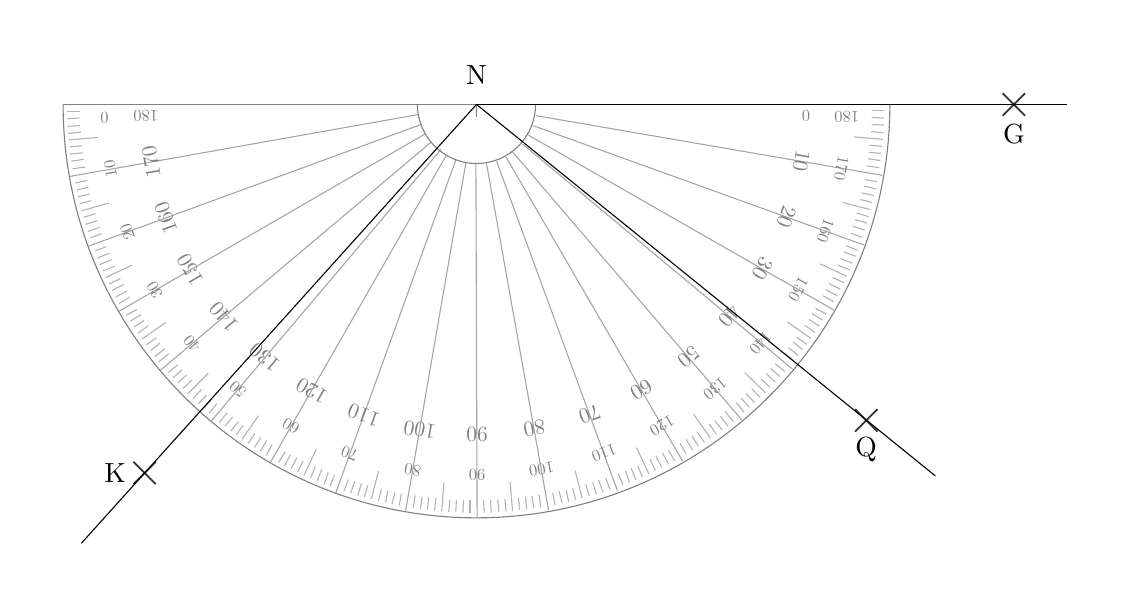
\begin{tikzpicture}[baseline,scale = 0.75]

\tikzset{
point/.style={
thick,
draw,
cross out,
inner sep=0pt,
minimum width=5pt,
minimum height=5pt,
},
}
\clip (-7.6,-7.93) rectangle (10.5,1.3);
\draw[color ={gray}] (-7,0)--(7,0);
\draw[color={gray}] (-1,0) arc (180:359.9:1) ;
\draw[color={gray}] (-7,0) arc (180:359.9:7) ;
\draw [color={gray}] (-5.6,-0.2) node[anchor = center,scale=0.6, rotate = 180] {180};
\draw [color={gray}] (-5.51,-0.97) node[anchor = center,scale=0.78, rotate = 100] {170};
\draw [color={gray}] (-6.3,-0.22) node[anchor = center,scale=0.6, rotate = 180] {0};
\draw [color={gray}] (-6.2,-1.09) node[anchor = center,scale=0.6, rotate = 100] {10};
\draw[color ={gray},opacity = 0.6] (-6.72,-0.12)--(-6.93,-0.12);
\draw[color ={gray},opacity = 0.6] (-6.72,-0.23)--(-6.93,-0.24);
\draw[color ={gray},opacity = 0.6] (-6.71,-0.36)--(-6.92,-0.37);
\draw[color ={gray},opacity = 0.6] (-6.7,-0.47)--(-6.91,-0.49);
\draw[color ={gray},opacity = 0.6] (-6.41,-0.56)--(-6.9,-0.6);
\draw[color ={gray},opacity = 0.6] (-6.68,-0.7)--(-6.89,-0.72);
\draw[color ={gray},opacity = 0.6] (-6.67,-0.82)--(-6.88,-0.84);
\draw[color ={gray},opacity = 0.6] (-6.65,-0.93)--(-6.86,-0.96);
\draw[color ={gray},opacity = 0.6] (-6.63,-1.06)--(-6.84,-1.09);
\draw [color={gray}] (-5.26,-1.92) node[anchor = center,scale=0.78, rotate = 110] {160};
\draw [color={gray}] (-5.91,-2.16) node[anchor = center,scale=0.6, rotate = 110] {20};
\draw[color ={gray},opacity = 0.6] (-6.6,-1.29)--(-6.8,-1.33);
\draw[color ={gray},opacity = 0.6] (-6.57,-1.4)--(-6.77,-1.45);
\draw[color ={gray},opacity = 0.6] (-6.55,-1.52)--(-6.75,-1.56);
\draw[color ={gray},opacity = 0.6] (-6.52,-1.63)--(-6.72,-1.68);
\draw[color ={gray},opacity = 0.6] (-6.22,-1.67)--(-6.69,-1.8);
\draw[color ={gray},opacity = 0.6] (-6.45,-1.85)--(-6.65,-1.91);
\draw[color ={gray},opacity = 0.6] (-6.42,-1.97)--(-6.62,-2.03);
\draw[color ={gray},opacity = 0.6] (-6.38,-2.08)--(-6.58,-2.15);
\draw[color ={gray},opacity = 0.6] (-6.35,-2.19)--(-6.54,-2.26);
\draw[color ={gray},opacity = 0.7] (-0.98,-0.17)--(-6.89,-1.22);
\draw [color={gray}] (-4.85,-2.8) node[anchor = center,scale=0.78, rotate = 120] {150};
\draw [color={gray}] (-5.45,-3.15) node[anchor = center,scale=0.6, rotate = 120] {30};
\draw[color ={gray},opacity = 0.6] (-6.27,-2.41)--(-6.46,-2.48);
\draw[color ={gray},opacity = 0.6] (-6.22,-2.52)--(-6.42,-2.6);
\draw[color ={gray},opacity = 0.6] (-6.18,-2.63)--(-6.38,-2.71);
\draw[color ={gray},opacity = 0.6] (-6.13,-2.74)--(-6.33,-2.82);
\draw[color ={gray},opacity = 0.6] (-5.83,-2.72)--(-6.28,-2.93);
\draw[color ={gray},opacity = 0.6] (-6.03,-2.95)--(-6.22,-3.04);
\draw[color ={gray},opacity = 0.6] (-5.98,-3.05)--(-6.17,-3.15);
\draw[color ={gray},opacity = 0.6] (-5.92,-3.16)--(-6.11,-3.26);
\draw[color ={gray},opacity = 0.6] (-5.87,-3.26)--(-6.05,-3.37);
\draw[color ={gray},opacity = 0.7] (-0.94,-0.34)--(-6.57,-2.4);
\draw [color={gray}] (-4.28,-3.6) node[anchor = center,scale=0.78, rotate = 130] {140};
\draw [color={gray}] (-4.82,-4.05) node[anchor = center,scale=0.6, rotate = 130] {40};
\draw[color ={gray},opacity = 0.6] (-5.75,-3.47)--(-5.93,-3.57);
\draw[color ={gray},opacity = 0.6] (-5.68,-3.56)--(-5.86,-3.67);
\draw[color ={gray},opacity = 0.6] (-5.63,-3.66)--(-5.8,-3.77);
\draw[color ={gray},opacity = 0.6] (-5.56,-3.75)--(-5.73,-3.87);
\draw[color ={gray},opacity = 0.6] (-5.26,-3.69)--(-5.66,-3.97);
\draw[color ={gray},opacity = 0.6] (-5.42,-3.95)--(-5.59,-4.07);
\draw[color ={gray},opacity = 0.6] (-5.36,-4.04)--(-5.52,-4.17);
\draw[color ={gray},opacity = 0.6] (-5.28,-4.14)--(-5.45,-4.27);
\draw[color ={gray},opacity = 0.6] (-5.21,-4.22)--(-5.38,-4.36);
\draw[color ={gray},opacity = 0.7] (-0.87,-0.5)--(-6.05,-3.5);
\draw [color={gray}] (-3.59,-4.29) node[anchor = center,scale=0.78, rotate = 140] {130};
\draw [color={gray}] (-4.04,-4.83) node[anchor = center,scale=0.6, rotate = 140] {50};
\draw[color ={gray},opacity = 0.6] (-5.06,-4.41)--(-5.22,-4.54);
\draw[color ={gray},opacity = 0.6] (-4.98,-4.49)--(-5.14,-4.63);
\draw[color ={gray},opacity = 0.6] (-4.91,-4.58)--(-5.06,-4.72);
\draw[color ={gray},opacity = 0.6] (-4.82,-4.67)--(-4.97,-4.81);
\draw[color ={gray},opacity = 0.6] (-4.54,-4.55)--(-4.89,-4.9);
\draw[color ={gray},opacity = 0.6] (-4.66,-4.83)--(-4.8,-4.98);
\draw[color ={gray},opacity = 0.6] (-4.57,-4.92)--(-4.71,-5.07);
\draw[color ={gray},opacity = 0.6] (-4.48,-4.99)--(-4.62,-5.15);
\draw[color ={gray},opacity = 0.6] (-4.4,-5.07)--(-4.53,-5.23);
\draw[color ={gray},opacity = 0.7] (-0.77,-0.64)--(-5.35,-4.5);
\draw [color={gray}] (-2.79,-4.85) node[anchor = center,scale=0.78, rotate = 150] {120};
\draw [color={gray}] (-3.14,-5.45) node[anchor = center,scale=0.6, rotate = 150] {60};
\draw[color ={gray},opacity = 0.6] (-4.22,-5.22)--(-4.36,-5.39);
\draw[color ={gray},opacity = 0.6] (-4.13,-5.29)--(-4.26,-5.45);
\draw[color ={gray},opacity = 0.6] (-4.03,-5.37)--(-4.16,-5.53);
\draw[color ={gray},opacity = 0.6] (-3.95,-5.43)--(-4.07,-5.6);
\draw[color ={gray},opacity = 0.6] (-3.69,-5.27)--(-3.97,-5.67);
\draw[color ={gray},opacity = 0.6] (-3.75,-5.57)--(-3.87,-5.74);
\draw[color ={gray},opacity = 0.6] (-3.65,-5.64)--(-3.76,-5.81);
\draw[color ={gray},opacity = 0.6] (-3.55,-5.69)--(-3.66,-5.87);
\draw[color ={gray},opacity = 0.6] (-3.46,-5.76)--(-3.56,-5.94);
\draw[color ={gray},opacity = 0.7] (-0.6,-0.76)--(-4.49,-5.36);
\draw [color={gray}] (-1.91,-5.26) node[anchor = center,scale=0.78, rotate = 160] {110};
\draw [color={gray}] (-2.15,-5.91) node[anchor = center,scale=0.6, rotate = 160] {70};
\draw[color ={gray},opacity = 0.6] (-3.24,-5.88)--(-3.35,-6.06);
\draw[color ={gray},opacity = 0.6] (-3.15,-5.93)--(-3.25,-6.12);
\draw[color ={gray},opacity = 0.6] (-3.04,-5.98)--(-3.14,-6.17);
\draw[color ={gray},opacity = 0.6] (-2.94,-6.04)--(-3.03,-6.23);
\draw[color ={gray},opacity = 0.6] (-2.71,-5.83)--(-2.92,-6.28);
\draw[color ={gray},opacity = 0.6] (-2.73,-6.13)--(-2.81,-6.33);
\draw[color ={gray},opacity = 0.6] (-2.62,-6.18)--(-2.7,-6.38);
\draw[color ={gray},opacity = 0.6] (-2.51,-6.23)--(-2.58,-6.43);
\draw[color ={gray},opacity = 0.6] (-2.4,-6.27)--(-2.48,-6.46);
\draw[color ={gray},opacity = 0.7] (-0.51,-0.86)--(-3.49,-6.06);
\draw [color={gray}] (-0.96,-5.51) node[anchor = center,scale=0.78, rotate = 170] {100};
\draw [color={gray}] (-1.08,-6.19) node[anchor = center,scale=0.6, rotate = 170] {80};
\draw[color ={gray},opacity = 0.6] (-2.17,-6.35)--(-2.24,-6.54);
\draw[color ={gray},opacity = 0.6] (-2.06,-6.38)--(-2.13,-6.58);
\draw[color ={gray},opacity = 0.6] (-1.95,-6.42)--(-2.01,-6.62);
\draw[color ={gray},opacity = 0.6] (-1.84,-6.45)--(-1.9,-6.65);
\draw[color ={gray},opacity = 0.6] (-1.66,-6.21)--(-1.78,-6.68);
\draw[color ={gray},opacity = 0.6] (-1.61,-6.51)--(-1.66,-6.71);
\draw[color ={gray},opacity = 0.6] (-1.5,-6.54)--(-1.54,-6.74);
\draw[color ={gray},opacity = 0.6] (-1.38,-6.57)--(-1.43,-6.77);
\draw[color ={gray},opacity = 0.6] (-1.27,-6.59)--(-1.31,-6.79);
\draw[color ={gray},opacity = 0.7] (-0.35,-0.94)--(-2.38,-6.57);
\draw [color={gray}] (0.01,-5.58) node[anchor = center,scale=0.78, rotate = 180] {90};
\draw [color={gray}] (0.01,-6.28) node[anchor = center,scale=0.6, rotate = 180] {90};
\draw[color ={gray},opacity = 0.6] (-1.04,-6.62)--(-1.07,-6.83);
\draw[color ={gray},opacity = 0.6] (-0.92,-6.64)--(-0.95,-6.85);
\draw[color ={gray},opacity = 0.6] (-0.81,-6.65)--(-0.83,-6.86);
\draw[color ={gray},opacity = 0.6] (-0.69,-6.67)--(-0.71,-6.88);
\draw[color ={gray},opacity = 0.6] (-0.55,-6.4)--(-0.59,-6.89);
\draw[color ={gray},opacity = 0.6] (-0.45,-6.69)--(-0.47,-6.9);
\draw[color ={gray},opacity = 0.6] (-0.34,-6.69)--(-0.35,-6.9);
\draw[color ={gray},opacity = 0.6] (-0.22,-6.7)--(-0.23,-6.91);
\draw[color ={gray},opacity = 0.6] (-0.11,-6.7)--(-0.11,-6.91);
\draw[color ={gray},opacity = 0.7] (-0.18,-0.99)--(-1.2,-6.88);
\draw [color={gray}] (0.98,-5.49) node[anchor = center,scale=0.78, rotate = 190] {80};
\draw [color={gray}] (1.1,-6.18) node[anchor = center,scale=0.6, rotate = 190] {100};
\draw[color ={gray},opacity = 0.6] (0.12,-6.7)--(0.13,-6.91);
\draw[color ={gray},opacity = 0.6] (0.24,-6.7)--(0.25,-6.91);
\draw[color ={gray},opacity = 0.6] (0.36,-6.69)--(0.38,-6.9);
\draw[color ={gray},opacity = 0.6] (0.48,-6.68)--(0.5,-6.89);
\draw[color ={gray},opacity = 0.6] (0.57,-6.39)--(0.61,-6.88);
\draw[color ={gray},opacity = 0.6] (0.71,-6.66)--(0.73,-6.87);
\draw[color ={gray},opacity = 0.6] (0.83,-6.65)--(0.85,-6.86);
\draw[color ={gray},opacity = 0.6] (0.94,-6.63)--(0.97,-6.84);
\draw[color ={gray},opacity = 0.6] (1.06,-6.61)--(1.09,-6.82);
\draw[color ={gray},opacity = 0.7] (-0.01,-1.01)--(0.01,-6.98);
\draw [color={gray}] (1.92,-5.25) node[anchor = center,scale=0.78, rotate = 200] {70};
\draw [color={gray}] (2.16,-5.9) node[anchor = center,scale=0.6, rotate = 200] {110};
\draw[color ={gray},opacity = 0.6] (1.29,-6.58)--(1.33,-6.78);
\draw[color ={gray},opacity = 0.6] (1.4,-6.55)--(1.45,-6.75);
\draw[color ={gray},opacity = 0.6] (1.52,-6.53)--(1.56,-6.73);
\draw[color ={gray},opacity = 0.6] (1.63,-6.5)--(1.68,-6.7);
\draw[color ={gray},opacity = 0.6] (1.67,-6.2)--(1.79,-6.67);
\draw[color ={gray},opacity = 0.6] (1.85,-6.43)--(1.91,-6.63);
\draw[color ={gray},opacity = 0.6] (1.97,-6.4)--(2.03,-6.6);
\draw[color ={gray},opacity = 0.6] (2.07,-6.36)--(2.14,-6.56);
\draw[color ={gray},opacity = 0.6] (2.19,-6.33)--(2.26,-6.52);
\draw[color ={gray},opacity = 0.7] (0.17,-1)--(1.22,-6.87);
\draw [color={gray}] (2.79,-4.83) node[anchor = center,scale=0.78, rotate = 210] {60};
\draw [color={gray}] (3.14,-5.44) node[anchor = center,scale=0.6, rotate = 210] {120};
\draw[color ={gray},opacity = 0.6] (2.4,-6.25)--(2.48,-6.44);
\draw[color ={gray},opacity = 0.6] (2.52,-6.2)--(2.59,-6.4);
\draw[color ={gray},opacity = 0.6] (2.62,-6.16)--(2.7,-6.36);
\draw[color ={gray},opacity = 0.6] (2.73,-6.12)--(2.81,-6.31);
\draw[color ={gray},opacity = 0.6] (2.71,-5.81)--(2.92,-6.26);
\draw[color ={gray},opacity = 0.6] (2.94,-6.01)--(3.03,-6.2);
\draw[color ={gray},opacity = 0.6] (3.04,-5.96)--(3.14,-6.15);
\draw[color ={gray},opacity = 0.6] (3.15,-5.9)--(3.25,-6.09);
\draw[color ={gray},opacity = 0.6] (3.25,-5.86)--(3.36,-6.04);
\draw[color ={gray},opacity = 0.7] (0.34,-0.96)--(2.39,-6.55);
\draw [color={gray}] (3.59,-4.27) node[anchor = center,scale=0.78, rotate = 220] {50};
\draw [color={gray}] (4.04,-4.81) node[anchor = center,scale=0.6, rotate = 220] {130};
\draw[color ={gray},opacity = 0.6] (3.45,-5.74)--(3.55,-5.92);
\draw[color ={gray},opacity = 0.6] (3.55,-5.67)--(3.66,-5.85);
\draw[color ={gray},opacity = 0.6] (3.65,-5.62)--(3.76,-5.79);
\draw[color ={gray},opacity = 0.6] (3.74,-5.55)--(3.86,-5.72);
\draw[color ={gray},opacity = 0.6] (3.68,-5.25)--(3.96,-5.65);
\draw[color ={gray},opacity = 0.6] (3.94,-5.41)--(4.06,-5.58);
\draw[color ={gray},opacity = 0.6] (4.03,-5.35)--(4.16,-5.51);
\draw[color ={gray},opacity = 0.6] (4.13,-5.28)--(4.26,-5.45);
\draw[color ={gray},opacity = 0.6] (4.21,-5.2)--(4.35,-5.37);
\draw[color ={gray},opacity = 0.7] (0.5,-0.89)--(3.49,-6.04);
\draw [color={gray}] (4.28,-3.58) node[anchor = center,scale=0.78, rotate = 230] {40};
\draw [color={gray}] (4.81,-4.04) node[anchor = center,scale=0.6, rotate = 230] {140};
\draw[color ={gray},opacity = 0.6] (4.4,-5.05)--(4.53,-5.21);
\draw[color ={gray},opacity = 0.6] (4.48,-4.97)--(4.62,-5.13);
\draw[color ={gray},opacity = 0.6] (4.57,-4.9)--(4.71,-5.05);
\draw[color ={gray},opacity = 0.6] (4.66,-4.81)--(4.8,-4.96);
\draw[color ={gray},opacity = 0.6] (4.54,-4.54)--(4.89,-4.88);
\draw[color ={gray},opacity = 0.6] (4.82,-4.65)--(4.97,-4.79);
\draw[color ={gray},opacity = 0.6] (4.91,-4.56)--(5.06,-4.7);
\draw[color ={gray},opacity = 0.6] (4.98,-4.47)--(5.14,-4.61);
\draw[color ={gray},opacity = 0.6] (5.06,-4.39)--(5.22,-4.52);
\draw[color ={gray},opacity = 0.7] (0.6,-0.79)--(4.49,-5.34);
\draw [color={gray}] (4.84,-2.78) node[anchor = center,scale=0.78, rotate = 240] {30};
\draw [color={gray}] (5.45,-3.13) node[anchor = center,scale=0.6, rotate = 240] {150};
\draw[color ={gray},opacity = 0.6] (5.21,-4.21)--(5.38,-4.35);
\draw[color ={gray},opacity = 0.6] (5.28,-4.12)--(5.45,-4.25);
\draw[color ={gray},opacity = 0.6] (5.36,-4.02)--(5.52,-4.15);
\draw[color ={gray},opacity = 0.6] (5.42,-3.94)--(5.59,-4.06);
\draw[color ={gray},opacity = 0.6] (5.26,-3.68)--(5.66,-3.96);
\draw[color ={gray},opacity = 0.6] (5.56,-3.74)--(5.73,-3.86);
\draw[color ={gray},opacity = 0.6] (5.63,-3.64)--(5.8,-3.75);
\draw[color ={gray},opacity = 0.6] (5.68,-3.54)--(5.86,-3.65);
\draw[color ={gray},opacity = 0.6] (5.74,-3.45)--(5.92,-3.55);
\draw[color ={gray},opacity = 0.7] (0.78,-0.67)--(5.35,-4.48);
\draw [color={gray}] (5.25,-1.9) node[anchor = center,scale=0.78, rotate = 250] {20};
\draw [color={gray}] (5.91,-2.14) node[anchor = center,scale=0.6, rotate = 250] {160};
\draw[color ={gray},opacity = 0.6] (5.87,-3.24)--(6.05,-3.34);
\draw[color ={gray},opacity = 0.6] (5.92,-3.14)--(6.11,-3.24);
\draw[color ={gray},opacity = 0.6] (5.97,-3.03)--(6.16,-3.13);
\draw[color ={gray},opacity = 0.6] (6.03,-2.93)--(6.22,-3.02);
\draw[color ={gray},opacity = 0.6] (5.82,-2.7)--(6.27,-2.91);
\draw[color ={gray},opacity = 0.6] (6.12,-2.72)--(6.32,-2.8);
\draw[color ={gray},opacity = 0.6] (6.17,-2.61)--(6.37,-2.69);
\draw[color ={gray},opacity = 0.6] (6.22,-2.5)--(6.42,-2.57);
\draw[color ={gray},opacity = 0.6] (6.26,-2.39)--(6.45,-2.47);
\draw[color ={gray},opacity = 0.7] (0.88,-0.52)--(6.05,-3.48);
\draw [color={gray}] (5.5,-0.96) node[anchor = center,scale=0.78, rotate = 260] {10};
\draw [color={gray}] (6.18,-1.08) node[anchor = center,scale=0.6, rotate = 260] {170};
\draw[color ={gray},opacity = 0.6] (6.34,-2.18)--(6.53,-2.25);
\draw[color ={gray},opacity = 0.6] (6.37,-2.06)--(6.57,-2.13);
\draw[color ={gray},opacity = 0.6] (6.41,-1.95)--(6.61,-2.01);
\draw[color ={gray},opacity = 0.6] (6.44,-1.84)--(6.64,-1.9);
\draw[color ={gray},opacity = 0.6] (6.2,-1.66)--(6.67,-1.78);
\draw[color ={gray},opacity = 0.6] (6.5,-1.61)--(6.7,-1.66);
\draw[color ={gray},opacity = 0.6] (6.53,-1.5)--(6.73,-1.54);
\draw[color ={gray},opacity = 0.6] (6.56,-1.38)--(6.76,-1.43);
\draw[color ={gray},opacity = 0.6] (6.58,-1.27)--(6.78,-1.31);
\draw[color ={gray},opacity = 0.7] (0.96,-0.36)--(6.56,-2.38);
\draw [color={gray}] (5.58,-0.19) node[anchor = center,scale=0.6, rotate = 180] {0};
\draw [color={gray}] (6.27,-0.21) node[anchor = center,scale=0.6, rotate = 180] {180};
\draw[color ={gray},opacity = 0.6] (6.61,-1.04)--(6.82,-1.07);
\draw[color ={gray},opacity = 0.6] (6.63,-0.92)--(6.84,-0.95);
\draw[color ={gray},opacity = 0.6] (6.64,-0.81)--(6.85,-0.83);
\draw[color ={gray},opacity = 0.6] (6.66,-0.69)--(6.87,-0.71);
\draw[color ={gray},opacity = 0.6] (6.39,-0.55)--(6.88,-0.59);
\draw[color ={gray},opacity = 0.6] (6.68,-0.46)--(6.89,-0.48);
\draw[color ={gray},opacity = 0.6] (6.69,-0.34)--(6.9,-0.35);
\draw[color ={gray},opacity = 0.6] (6.69,-0.22)--(6.9,-0.23);
\draw[color ={gray},opacity = 0.6] (6.69,-0.11)--(6.9,-0.11);
\draw[color ={gray},opacity = 0.7] (1.01,-0.19)--(6.87,-1.2);
\draw[color ={gray}] (0,0)--(0,-0.21);
\draw[color ={black}] (0,0)--(10,0);
\draw[color ={black}] (0,0)--(7.77,-6.29);
\draw [color={black}] (0,0.5) node[anchor = center,scale=1, rotate = 0] {N};
\draw [color={black}] (9.1,-0.5) node[anchor = center,scale=1, rotate = 0] {G};
\draw [color={black}] (6.6,-5.85) node[anchor = center,scale=1, rotate = 0] {Q};
\draw[color ={black},line width = 0.625,opacity = 0.8] (8.91,0.19)--(9.29,-0.19);\draw[color ={black},line width = 0.625,opacity = 0.8] (8.91,-0.19)--(9.29,0.19);\draw[color ={black},line width = 0.625,opacity = 0.8] (6.41,-5.16)--(6.79,-5.54);\draw[color ={black},line width = 0.625,opacity = 0.8] (6.41,-5.54)--(6.79,-5.16);
\draw[color ={black}] (0,0)--(-6.69,-7.43);
\draw [color={black}] (-6.12,-6.24) node[anchor = center,scale=1, rotate = 0] {K};
\draw[color ={black},line width = 0.625,opacity = 0.8] (-5.81,-6.05)--(-5.43,-6.43);\draw[color ={black},line width = 0.625,opacity = 0.8] (-5.81,-6.43)--(-5.43,-6.05);

\end{tikzpicture}\\
\item \textbf {a.}  Quelle est la mesure, en degrés, de l'angle $\widehat{MGT}$ ?\\\textbf {b.}  Quelle est la mesure, en degrés, de l'angle $\widehat{TGV}$ ?\\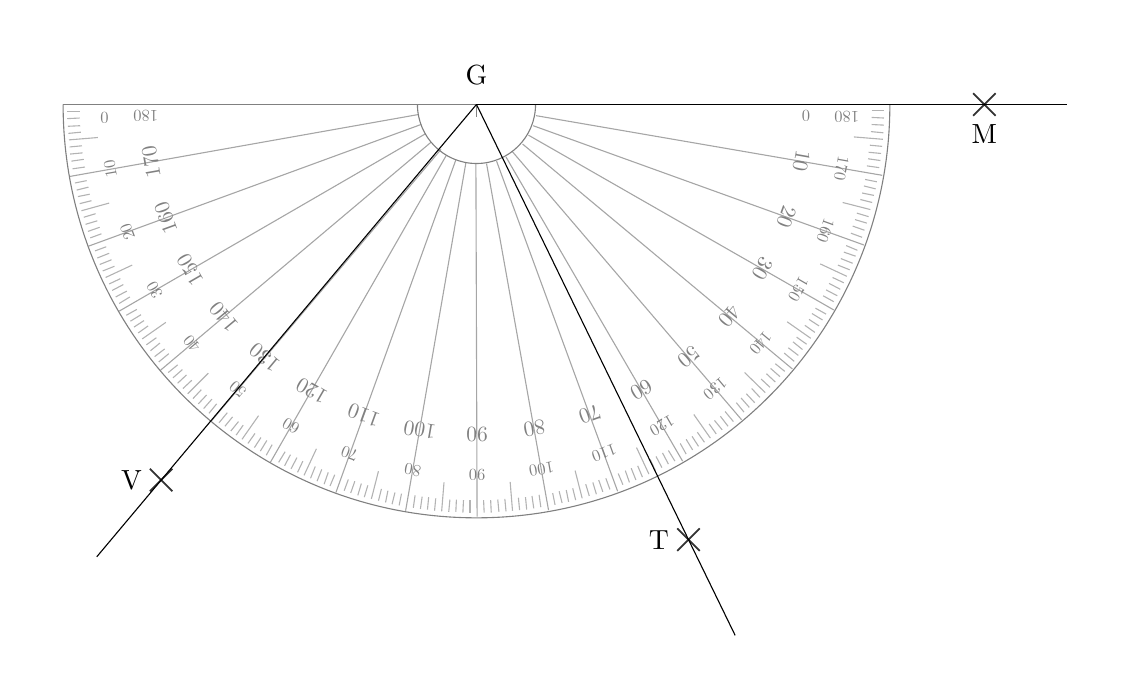
\begin{tikzpicture}[baseline,scale = 0.75]

\tikzset{
point/.style={
thick,
draw,
cross out,
inner sep=0pt,
minimum width=5pt,
minimum height=5pt,
},
}
\clip (-7.6,-9.49) rectangle (10.5,1.3);
\draw[color ={gray}] (-7,0)--(7,0);
\draw[color={gray}] (-1,0) arc (180:359.9:1) ;
\draw[color={gray}] (-7,0) arc (180:359.9:7) ;
\draw [color={gray}] (-5.6,-0.2) node[anchor = center,scale=0.6, rotate = 180] {180};
\draw [color={gray}] (-5.51,-0.97) node[anchor = center,scale=0.78, rotate = 100] {170};
\draw [color={gray}] (-6.3,-0.22) node[anchor = center,scale=0.6, rotate = 180] {0};
\draw [color={gray}] (-6.2,-1.09) node[anchor = center,scale=0.6, rotate = 100] {10};
\draw[color ={gray},opacity = 0.6] (-6.72,-0.12)--(-6.93,-0.12);
\draw[color ={gray},opacity = 0.6] (-6.72,-0.23)--(-6.93,-0.24);
\draw[color ={gray},opacity = 0.6] (-6.71,-0.36)--(-6.92,-0.37);
\draw[color ={gray},opacity = 0.6] (-6.7,-0.47)--(-6.91,-0.49);
\draw[color ={gray},opacity = 0.6] (-6.41,-0.56)--(-6.9,-0.6);
\draw[color ={gray},opacity = 0.6] (-6.68,-0.7)--(-6.89,-0.72);
\draw[color ={gray},opacity = 0.6] (-6.67,-0.82)--(-6.88,-0.84);
\draw[color ={gray},opacity = 0.6] (-6.65,-0.93)--(-6.86,-0.96);
\draw[color ={gray},opacity = 0.6] (-6.63,-1.06)--(-6.84,-1.09);
\draw [color={gray}] (-5.26,-1.92) node[anchor = center,scale=0.78, rotate = 110] {160};
\draw [color={gray}] (-5.91,-2.16) node[anchor = center,scale=0.6, rotate = 110] {20};
\draw[color ={gray},opacity = 0.6] (-6.6,-1.29)--(-6.8,-1.33);
\draw[color ={gray},opacity = 0.6] (-6.57,-1.4)--(-6.77,-1.45);
\draw[color ={gray},opacity = 0.6] (-6.55,-1.52)--(-6.75,-1.56);
\draw[color ={gray},opacity = 0.6] (-6.52,-1.63)--(-6.72,-1.68);
\draw[color ={gray},opacity = 0.6] (-6.22,-1.67)--(-6.69,-1.8);
\draw[color ={gray},opacity = 0.6] (-6.45,-1.85)--(-6.65,-1.91);
\draw[color ={gray},opacity = 0.6] (-6.42,-1.97)--(-6.62,-2.03);
\draw[color ={gray},opacity = 0.6] (-6.38,-2.08)--(-6.58,-2.15);
\draw[color ={gray},opacity = 0.6] (-6.35,-2.19)--(-6.54,-2.26);
\draw[color ={gray},opacity = 0.7] (-0.98,-0.17)--(-6.89,-1.22);
\draw [color={gray}] (-4.85,-2.8) node[anchor = center,scale=0.78, rotate = 120] {150};
\draw [color={gray}] (-5.45,-3.15) node[anchor = center,scale=0.6, rotate = 120] {30};
\draw[color ={gray},opacity = 0.6] (-6.27,-2.41)--(-6.46,-2.48);
\draw[color ={gray},opacity = 0.6] (-6.22,-2.52)--(-6.42,-2.6);
\draw[color ={gray},opacity = 0.6] (-6.18,-2.63)--(-6.38,-2.71);
\draw[color ={gray},opacity = 0.6] (-6.13,-2.74)--(-6.33,-2.82);
\draw[color ={gray},opacity = 0.6] (-5.83,-2.72)--(-6.28,-2.93);
\draw[color ={gray},opacity = 0.6] (-6.03,-2.95)--(-6.22,-3.04);
\draw[color ={gray},opacity = 0.6] (-5.98,-3.05)--(-6.17,-3.15);
\draw[color ={gray},opacity = 0.6] (-5.92,-3.16)--(-6.11,-3.26);
\draw[color ={gray},opacity = 0.6] (-5.87,-3.26)--(-6.05,-3.37);
\draw[color ={gray},opacity = 0.7] (-0.94,-0.34)--(-6.57,-2.4);
\draw [color={gray}] (-4.28,-3.6) node[anchor = center,scale=0.78, rotate = 130] {140};
\draw [color={gray}] (-4.82,-4.05) node[anchor = center,scale=0.6, rotate = 130] {40};
\draw[color ={gray},opacity = 0.6] (-5.75,-3.47)--(-5.93,-3.57);
\draw[color ={gray},opacity = 0.6] (-5.68,-3.56)--(-5.86,-3.67);
\draw[color ={gray},opacity = 0.6] (-5.63,-3.66)--(-5.8,-3.77);
\draw[color ={gray},opacity = 0.6] (-5.56,-3.75)--(-5.73,-3.87);
\draw[color ={gray},opacity = 0.6] (-5.26,-3.69)--(-5.66,-3.97);
\draw[color ={gray},opacity = 0.6] (-5.42,-3.95)--(-5.59,-4.07);
\draw[color ={gray},opacity = 0.6] (-5.36,-4.04)--(-5.52,-4.17);
\draw[color ={gray},opacity = 0.6] (-5.28,-4.14)--(-5.45,-4.27);
\draw[color ={gray},opacity = 0.6] (-5.21,-4.22)--(-5.38,-4.36);
\draw[color ={gray},opacity = 0.7] (-0.87,-0.5)--(-6.05,-3.5);
\draw [color={gray}] (-3.59,-4.29) node[anchor = center,scale=0.78, rotate = 140] {130};
\draw [color={gray}] (-4.04,-4.83) node[anchor = center,scale=0.6, rotate = 140] {50};
\draw[color ={gray},opacity = 0.6] (-5.06,-4.41)--(-5.22,-4.54);
\draw[color ={gray},opacity = 0.6] (-4.98,-4.49)--(-5.14,-4.63);
\draw[color ={gray},opacity = 0.6] (-4.91,-4.58)--(-5.06,-4.72);
\draw[color ={gray},opacity = 0.6] (-4.82,-4.67)--(-4.97,-4.81);
\draw[color ={gray},opacity = 0.6] (-4.54,-4.55)--(-4.89,-4.9);
\draw[color ={gray},opacity = 0.6] (-4.66,-4.83)--(-4.8,-4.98);
\draw[color ={gray},opacity = 0.6] (-4.57,-4.92)--(-4.71,-5.07);
\draw[color ={gray},opacity = 0.6] (-4.48,-4.99)--(-4.62,-5.15);
\draw[color ={gray},opacity = 0.6] (-4.4,-5.07)--(-4.53,-5.23);
\draw[color ={gray},opacity = 0.7] (-0.77,-0.64)--(-5.35,-4.5);
\draw [color={gray}] (-2.79,-4.85) node[anchor = center,scale=0.78, rotate = 150] {120};
\draw [color={gray}] (-3.14,-5.45) node[anchor = center,scale=0.6, rotate = 150] {60};
\draw[color ={gray},opacity = 0.6] (-4.22,-5.22)--(-4.36,-5.39);
\draw[color ={gray},opacity = 0.6] (-4.13,-5.29)--(-4.26,-5.45);
\draw[color ={gray},opacity = 0.6] (-4.03,-5.37)--(-4.16,-5.53);
\draw[color ={gray},opacity = 0.6] (-3.95,-5.43)--(-4.07,-5.6);
\draw[color ={gray},opacity = 0.6] (-3.69,-5.27)--(-3.97,-5.67);
\draw[color ={gray},opacity = 0.6] (-3.75,-5.57)--(-3.87,-5.74);
\draw[color ={gray},opacity = 0.6] (-3.65,-5.64)--(-3.76,-5.81);
\draw[color ={gray},opacity = 0.6] (-3.55,-5.69)--(-3.66,-5.87);
\draw[color ={gray},opacity = 0.6] (-3.46,-5.76)--(-3.56,-5.94);
\draw[color ={gray},opacity = 0.7] (-0.6,-0.76)--(-4.49,-5.36);
\draw [color={gray}] (-1.91,-5.26) node[anchor = center,scale=0.78, rotate = 160] {110};
\draw [color={gray}] (-2.15,-5.91) node[anchor = center,scale=0.6, rotate = 160] {70};
\draw[color ={gray},opacity = 0.6] (-3.24,-5.88)--(-3.35,-6.06);
\draw[color ={gray},opacity = 0.6] (-3.15,-5.93)--(-3.25,-6.12);
\draw[color ={gray},opacity = 0.6] (-3.04,-5.98)--(-3.14,-6.17);
\draw[color ={gray},opacity = 0.6] (-2.94,-6.04)--(-3.03,-6.23);
\draw[color ={gray},opacity = 0.6] (-2.71,-5.83)--(-2.92,-6.28);
\draw[color ={gray},opacity = 0.6] (-2.73,-6.13)--(-2.81,-6.33);
\draw[color ={gray},opacity = 0.6] (-2.62,-6.18)--(-2.7,-6.38);
\draw[color ={gray},opacity = 0.6] (-2.51,-6.23)--(-2.58,-6.43);
\draw[color ={gray},opacity = 0.6] (-2.4,-6.27)--(-2.48,-6.46);
\draw[color ={gray},opacity = 0.7] (-0.51,-0.86)--(-3.49,-6.06);
\draw [color={gray}] (-0.96,-5.51) node[anchor = center,scale=0.78, rotate = 170] {100};
\draw [color={gray}] (-1.08,-6.19) node[anchor = center,scale=0.6, rotate = 170] {80};
\draw[color ={gray},opacity = 0.6] (-2.17,-6.35)--(-2.24,-6.54);
\draw[color ={gray},opacity = 0.6] (-2.06,-6.38)--(-2.13,-6.58);
\draw[color ={gray},opacity = 0.6] (-1.95,-6.42)--(-2.01,-6.62);
\draw[color ={gray},opacity = 0.6] (-1.84,-6.45)--(-1.9,-6.65);
\draw[color ={gray},opacity = 0.6] (-1.66,-6.21)--(-1.78,-6.68);
\draw[color ={gray},opacity = 0.6] (-1.61,-6.51)--(-1.66,-6.71);
\draw[color ={gray},opacity = 0.6] (-1.5,-6.54)--(-1.54,-6.74);
\draw[color ={gray},opacity = 0.6] (-1.38,-6.57)--(-1.43,-6.77);
\draw[color ={gray},opacity = 0.6] (-1.27,-6.59)--(-1.31,-6.79);
\draw[color ={gray},opacity = 0.7] (-0.35,-0.94)--(-2.38,-6.57);
\draw [color={gray}] (0.01,-5.58) node[anchor = center,scale=0.78, rotate = 180] {90};
\draw [color={gray}] (0.01,-6.28) node[anchor = center,scale=0.6, rotate = 180] {90};
\draw[color ={gray},opacity = 0.6] (-1.04,-6.62)--(-1.07,-6.83);
\draw[color ={gray},opacity = 0.6] (-0.92,-6.64)--(-0.95,-6.85);
\draw[color ={gray},opacity = 0.6] (-0.81,-6.65)--(-0.83,-6.86);
\draw[color ={gray},opacity = 0.6] (-0.69,-6.67)--(-0.71,-6.88);
\draw[color ={gray},opacity = 0.6] (-0.55,-6.4)--(-0.59,-6.89);
\draw[color ={gray},opacity = 0.6] (-0.45,-6.69)--(-0.47,-6.9);
\draw[color ={gray},opacity = 0.6] (-0.34,-6.69)--(-0.35,-6.9);
\draw[color ={gray},opacity = 0.6] (-0.22,-6.7)--(-0.23,-6.91);
\draw[color ={gray},opacity = 0.6] (-0.11,-6.7)--(-0.11,-6.91);
\draw[color ={gray},opacity = 0.7] (-0.18,-0.99)--(-1.2,-6.88);
\draw [color={gray}] (0.98,-5.49) node[anchor = center,scale=0.78, rotate = 190] {80};
\draw [color={gray}] (1.1,-6.18) node[anchor = center,scale=0.6, rotate = 190] {100};
\draw[color ={gray},opacity = 0.6] (0.12,-6.7)--(0.13,-6.91);
\draw[color ={gray},opacity = 0.6] (0.24,-6.7)--(0.25,-6.91);
\draw[color ={gray},opacity = 0.6] (0.36,-6.69)--(0.38,-6.9);
\draw[color ={gray},opacity = 0.6] (0.48,-6.68)--(0.5,-6.89);
\draw[color ={gray},opacity = 0.6] (0.57,-6.39)--(0.61,-6.88);
\draw[color ={gray},opacity = 0.6] (0.71,-6.66)--(0.73,-6.87);
\draw[color ={gray},opacity = 0.6] (0.83,-6.65)--(0.85,-6.86);
\draw[color ={gray},opacity = 0.6] (0.94,-6.63)--(0.97,-6.84);
\draw[color ={gray},opacity = 0.6] (1.06,-6.61)--(1.09,-6.82);
\draw[color ={gray},opacity = 0.7] (-0.01,-1.01)--(0.01,-6.98);
\draw [color={gray}] (1.92,-5.25) node[anchor = center,scale=0.78, rotate = 200] {70};
\draw [color={gray}] (2.16,-5.9) node[anchor = center,scale=0.6, rotate = 200] {110};
\draw[color ={gray},opacity = 0.6] (1.29,-6.58)--(1.33,-6.78);
\draw[color ={gray},opacity = 0.6] (1.4,-6.55)--(1.45,-6.75);
\draw[color ={gray},opacity = 0.6] (1.52,-6.53)--(1.56,-6.73);
\draw[color ={gray},opacity = 0.6] (1.63,-6.5)--(1.68,-6.7);
\draw[color ={gray},opacity = 0.6] (1.67,-6.2)--(1.79,-6.67);
\draw[color ={gray},opacity = 0.6] (1.85,-6.43)--(1.91,-6.63);
\draw[color ={gray},opacity = 0.6] (1.97,-6.4)--(2.03,-6.6);
\draw[color ={gray},opacity = 0.6] (2.07,-6.36)--(2.14,-6.56);
\draw[color ={gray},opacity = 0.6] (2.19,-6.33)--(2.26,-6.52);
\draw[color ={gray},opacity = 0.7] (0.17,-1)--(1.22,-6.87);
\draw [color={gray}] (2.79,-4.83) node[anchor = center,scale=0.78, rotate = 210] {60};
\draw [color={gray}] (3.14,-5.44) node[anchor = center,scale=0.6, rotate = 210] {120};
\draw[color ={gray},opacity = 0.6] (2.4,-6.25)--(2.48,-6.44);
\draw[color ={gray},opacity = 0.6] (2.52,-6.2)--(2.59,-6.4);
\draw[color ={gray},opacity = 0.6] (2.62,-6.16)--(2.7,-6.36);
\draw[color ={gray},opacity = 0.6] (2.73,-6.12)--(2.81,-6.31);
\draw[color ={gray},opacity = 0.6] (2.71,-5.81)--(2.92,-6.26);
\draw[color ={gray},opacity = 0.6] (2.94,-6.01)--(3.03,-6.2);
\draw[color ={gray},opacity = 0.6] (3.04,-5.96)--(3.14,-6.15);
\draw[color ={gray},opacity = 0.6] (3.15,-5.9)--(3.25,-6.09);
\draw[color ={gray},opacity = 0.6] (3.25,-5.86)--(3.36,-6.04);
\draw[color ={gray},opacity = 0.7] (0.34,-0.96)--(2.39,-6.55);
\draw [color={gray}] (3.59,-4.27) node[anchor = center,scale=0.78, rotate = 220] {50};
\draw [color={gray}] (4.04,-4.81) node[anchor = center,scale=0.6, rotate = 220] {130};
\draw[color ={gray},opacity = 0.6] (3.45,-5.74)--(3.55,-5.92);
\draw[color ={gray},opacity = 0.6] (3.55,-5.67)--(3.66,-5.85);
\draw[color ={gray},opacity = 0.6] (3.65,-5.62)--(3.76,-5.79);
\draw[color ={gray},opacity = 0.6] (3.74,-5.55)--(3.86,-5.72);
\draw[color ={gray},opacity = 0.6] (3.68,-5.25)--(3.96,-5.65);
\draw[color ={gray},opacity = 0.6] (3.94,-5.41)--(4.06,-5.58);
\draw[color ={gray},opacity = 0.6] (4.03,-5.35)--(4.16,-5.51);
\draw[color ={gray},opacity = 0.6] (4.13,-5.28)--(4.26,-5.45);
\draw[color ={gray},opacity = 0.6] (4.21,-5.2)--(4.35,-5.37);
\draw[color ={gray},opacity = 0.7] (0.5,-0.89)--(3.49,-6.04);
\draw [color={gray}] (4.28,-3.58) node[anchor = center,scale=0.78, rotate = 230] {40};
\draw [color={gray}] (4.81,-4.04) node[anchor = center,scale=0.6, rotate = 230] {140};
\draw[color ={gray},opacity = 0.6] (4.4,-5.05)--(4.53,-5.21);
\draw[color ={gray},opacity = 0.6] (4.48,-4.97)--(4.62,-5.13);
\draw[color ={gray},opacity = 0.6] (4.57,-4.9)--(4.71,-5.05);
\draw[color ={gray},opacity = 0.6] (4.66,-4.81)--(4.8,-4.96);
\draw[color ={gray},opacity = 0.6] (4.54,-4.54)--(4.89,-4.88);
\draw[color ={gray},opacity = 0.6] (4.82,-4.65)--(4.97,-4.79);
\draw[color ={gray},opacity = 0.6] (4.91,-4.56)--(5.06,-4.7);
\draw[color ={gray},opacity = 0.6] (4.98,-4.47)--(5.14,-4.61);
\draw[color ={gray},opacity = 0.6] (5.06,-4.39)--(5.22,-4.52);
\draw[color ={gray},opacity = 0.7] (0.6,-0.79)--(4.49,-5.34);
\draw [color={gray}] (4.84,-2.78) node[anchor = center,scale=0.78, rotate = 240] {30};
\draw [color={gray}] (5.45,-3.13) node[anchor = center,scale=0.6, rotate = 240] {150};
\draw[color ={gray},opacity = 0.6] (5.21,-4.21)--(5.38,-4.35);
\draw[color ={gray},opacity = 0.6] (5.28,-4.12)--(5.45,-4.25);
\draw[color ={gray},opacity = 0.6] (5.36,-4.02)--(5.52,-4.15);
\draw[color ={gray},opacity = 0.6] (5.42,-3.94)--(5.59,-4.06);
\draw[color ={gray},opacity = 0.6] (5.26,-3.68)--(5.66,-3.96);
\draw[color ={gray},opacity = 0.6] (5.56,-3.74)--(5.73,-3.86);
\draw[color ={gray},opacity = 0.6] (5.63,-3.64)--(5.8,-3.75);
\draw[color ={gray},opacity = 0.6] (5.68,-3.54)--(5.86,-3.65);
\draw[color ={gray},opacity = 0.6] (5.74,-3.45)--(5.92,-3.55);
\draw[color ={gray},opacity = 0.7] (0.78,-0.67)--(5.35,-4.48);
\draw [color={gray}] (5.25,-1.9) node[anchor = center,scale=0.78, rotate = 250] {20};
\draw [color={gray}] (5.91,-2.14) node[anchor = center,scale=0.6, rotate = 250] {160};
\draw[color ={gray},opacity = 0.6] (5.87,-3.24)--(6.05,-3.34);
\draw[color ={gray},opacity = 0.6] (5.92,-3.14)--(6.11,-3.24);
\draw[color ={gray},opacity = 0.6] (5.97,-3.03)--(6.16,-3.13);
\draw[color ={gray},opacity = 0.6] (6.03,-2.93)--(6.22,-3.02);
\draw[color ={gray},opacity = 0.6] (5.82,-2.7)--(6.27,-2.91);
\draw[color ={gray},opacity = 0.6] (6.12,-2.72)--(6.32,-2.8);
\draw[color ={gray},opacity = 0.6] (6.17,-2.61)--(6.37,-2.69);
\draw[color ={gray},opacity = 0.6] (6.22,-2.5)--(6.42,-2.57);
\draw[color ={gray},opacity = 0.6] (6.26,-2.39)--(6.45,-2.47);
\draw[color ={gray},opacity = 0.7] (0.88,-0.52)--(6.05,-3.48);
\draw [color={gray}] (5.5,-0.96) node[anchor = center,scale=0.78, rotate = 260] {10};
\draw [color={gray}] (6.18,-1.08) node[anchor = center,scale=0.6, rotate = 260] {170};
\draw[color ={gray},opacity = 0.6] (6.34,-2.18)--(6.53,-2.25);
\draw[color ={gray},opacity = 0.6] (6.37,-2.06)--(6.57,-2.13);
\draw[color ={gray},opacity = 0.6] (6.41,-1.95)--(6.61,-2.01);
\draw[color ={gray},opacity = 0.6] (6.44,-1.84)--(6.64,-1.9);
\draw[color ={gray},opacity = 0.6] (6.2,-1.66)--(6.67,-1.78);
\draw[color ={gray},opacity = 0.6] (6.5,-1.61)--(6.7,-1.66);
\draw[color ={gray},opacity = 0.6] (6.53,-1.5)--(6.73,-1.54);
\draw[color ={gray},opacity = 0.6] (6.56,-1.38)--(6.76,-1.43);
\draw[color ={gray},opacity = 0.6] (6.58,-1.27)--(6.78,-1.31);
\draw[color ={gray},opacity = 0.7] (0.96,-0.36)--(6.56,-2.38);
\draw [color={gray}] (5.58,-0.19) node[anchor = center,scale=0.6, rotate = 180] {0};
\draw [color={gray}] (6.27,-0.21) node[anchor = center,scale=0.6, rotate = 180] {180};
\draw[color ={gray},opacity = 0.6] (6.61,-1.04)--(6.82,-1.07);
\draw[color ={gray},opacity = 0.6] (6.63,-0.92)--(6.84,-0.95);
\draw[color ={gray},opacity = 0.6] (6.64,-0.81)--(6.85,-0.83);
\draw[color ={gray},opacity = 0.6] (6.66,-0.69)--(6.87,-0.71);
\draw[color ={gray},opacity = 0.6] (6.39,-0.55)--(6.88,-0.59);
\draw[color ={gray},opacity = 0.6] (6.68,-0.46)--(6.89,-0.48);
\draw[color ={gray},opacity = 0.6] (6.69,-0.34)--(6.9,-0.35);
\draw[color ={gray},opacity = 0.6] (6.69,-0.22)--(6.9,-0.23);
\draw[color ={gray},opacity = 0.6] (6.69,-0.11)--(6.9,-0.11);
\draw[color ={gray},opacity = 0.7] (1.01,-0.19)--(6.87,-1.2);
\draw[color ={gray}] (0,0)--(0,-0.21);
\draw[color ={black}] (0,0)--(10,0);
\draw[color ={black}] (0,0)--(4.38,-8.99);
\draw [color={black}] (0,0.5) node[anchor = center,scale=1, rotate = 0] {G};
\draw [color={black}] (8.6,-0.5) node[anchor = center,scale=1, rotate = 0] {M};
\draw [color={black}] (3.09,-7.37) node[anchor = center,scale=1, rotate = 0] {T};
\draw[color ={black},line width = 0.625,opacity = 0.8] (8.41,0.19)--(8.79,-0.19);\draw[color ={black},line width = 0.625,opacity = 0.8] (8.41,-0.19)--(8.79,0.19);\draw[color ={black},line width = 0.625,opacity = 0.8] (3.4,-7.18)--(3.78,-7.56);\draw[color ={black},line width = 0.625,opacity = 0.8] (3.4,-7.56)--(3.78,-7.18);
\draw[color ={black}] (0,0)--(-6.43,-7.66);
\draw [color={black}] (-5.84,-6.36) node[anchor = center,scale=1, rotate = 0] {V};
\draw[color ={black},line width = 0.625,opacity = 0.8] (-5.53,-6.17)--(-5.15,-6.55);\draw[color ={black},line width = 0.625,opacity = 0.8] (-5.53,-6.55)--(-5.15,-6.17);

\end{tikzpicture}\\
\item \textbf {a.}  Quelle est la mesure, en degrés, de l'angle $\widehat{NVZ}$ ?\\\textbf {b.}  Quelle est la mesure, en degrés, de l'angle $\widehat{ZVK}$ ?\\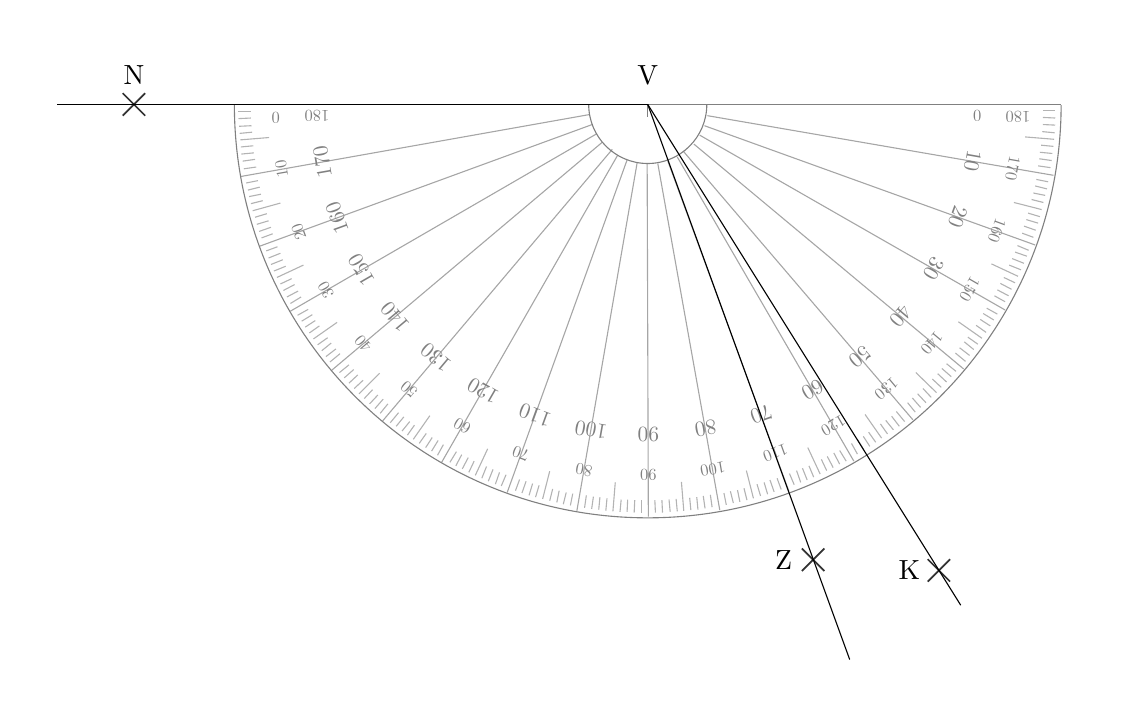
\begin{tikzpicture}[baseline,scale = 0.75]

\tikzset{
point/.style={
thick,
draw,
cross out,
inner sep=0pt,
minimum width=5pt,
minimum height=5pt,
},
}
\clip (-10.5,-9.9) rectangle (7.6,1.3);
\draw[color ={gray}] (-7,0)--(7,0);
\draw[color={gray}] (-1,0) arc (180:359.9:1) ;
\draw[color={gray}] (-7,0) arc (180:359.9:7) ;
\draw [color={gray}] (-5.6,-0.2) node[anchor = center,scale=0.6, rotate = 180] {180};
\draw [color={gray}] (-5.51,-0.97) node[anchor = center,scale=0.78, rotate = 100] {170};
\draw [color={gray}] (-6.3,-0.22) node[anchor = center,scale=0.6, rotate = 180] {0};
\draw [color={gray}] (-6.2,-1.09) node[anchor = center,scale=0.6, rotate = 100] {10};
\draw[color ={gray},opacity = 0.6] (-6.72,-0.12)--(-6.93,-0.12);
\draw[color ={gray},opacity = 0.6] (-6.72,-0.23)--(-6.93,-0.24);
\draw[color ={gray},opacity = 0.6] (-6.71,-0.36)--(-6.92,-0.37);
\draw[color ={gray},opacity = 0.6] (-6.7,-0.47)--(-6.91,-0.49);
\draw[color ={gray},opacity = 0.6] (-6.41,-0.56)--(-6.9,-0.6);
\draw[color ={gray},opacity = 0.6] (-6.68,-0.7)--(-6.89,-0.72);
\draw[color ={gray},opacity = 0.6] (-6.67,-0.82)--(-6.88,-0.84);
\draw[color ={gray},opacity = 0.6] (-6.65,-0.93)--(-6.86,-0.96);
\draw[color ={gray},opacity = 0.6] (-6.63,-1.06)--(-6.84,-1.09);
\draw [color={gray}] (-5.26,-1.92) node[anchor = center,scale=0.78, rotate = 110] {160};
\draw [color={gray}] (-5.91,-2.16) node[anchor = center,scale=0.6, rotate = 110] {20};
\draw[color ={gray},opacity = 0.6] (-6.6,-1.29)--(-6.8,-1.33);
\draw[color ={gray},opacity = 0.6] (-6.57,-1.4)--(-6.77,-1.45);
\draw[color ={gray},opacity = 0.6] (-6.55,-1.52)--(-6.75,-1.56);
\draw[color ={gray},opacity = 0.6] (-6.52,-1.63)--(-6.72,-1.68);
\draw[color ={gray},opacity = 0.6] (-6.22,-1.67)--(-6.69,-1.8);
\draw[color ={gray},opacity = 0.6] (-6.45,-1.85)--(-6.65,-1.91);
\draw[color ={gray},opacity = 0.6] (-6.42,-1.97)--(-6.62,-2.03);
\draw[color ={gray},opacity = 0.6] (-6.38,-2.08)--(-6.58,-2.15);
\draw[color ={gray},opacity = 0.6] (-6.35,-2.19)--(-6.54,-2.26);
\draw[color ={gray},opacity = 0.7] (-0.98,-0.17)--(-6.89,-1.22);
\draw [color={gray}] (-4.85,-2.8) node[anchor = center,scale=0.78, rotate = 120] {150};
\draw [color={gray}] (-5.45,-3.15) node[anchor = center,scale=0.6, rotate = 120] {30};
\draw[color ={gray},opacity = 0.6] (-6.27,-2.41)--(-6.46,-2.48);
\draw[color ={gray},opacity = 0.6] (-6.22,-2.52)--(-6.42,-2.6);
\draw[color ={gray},opacity = 0.6] (-6.18,-2.63)--(-6.38,-2.71);
\draw[color ={gray},opacity = 0.6] (-6.13,-2.74)--(-6.33,-2.82);
\draw[color ={gray},opacity = 0.6] (-5.83,-2.72)--(-6.28,-2.93);
\draw[color ={gray},opacity = 0.6] (-6.03,-2.95)--(-6.22,-3.04);
\draw[color ={gray},opacity = 0.6] (-5.98,-3.05)--(-6.17,-3.15);
\draw[color ={gray},opacity = 0.6] (-5.92,-3.16)--(-6.11,-3.26);
\draw[color ={gray},opacity = 0.6] (-5.87,-3.26)--(-6.05,-3.37);
\draw[color ={gray},opacity = 0.7] (-0.94,-0.34)--(-6.57,-2.4);
\draw [color={gray}] (-4.28,-3.6) node[anchor = center,scale=0.78, rotate = 130] {140};
\draw [color={gray}] (-4.82,-4.05) node[anchor = center,scale=0.6, rotate = 130] {40};
\draw[color ={gray},opacity = 0.6] (-5.75,-3.47)--(-5.93,-3.57);
\draw[color ={gray},opacity = 0.6] (-5.68,-3.56)--(-5.86,-3.67);
\draw[color ={gray},opacity = 0.6] (-5.63,-3.66)--(-5.8,-3.77);
\draw[color ={gray},opacity = 0.6] (-5.56,-3.75)--(-5.73,-3.87);
\draw[color ={gray},opacity = 0.6] (-5.26,-3.69)--(-5.66,-3.97);
\draw[color ={gray},opacity = 0.6] (-5.42,-3.95)--(-5.59,-4.07);
\draw[color ={gray},opacity = 0.6] (-5.36,-4.04)--(-5.52,-4.17);
\draw[color ={gray},opacity = 0.6] (-5.28,-4.14)--(-5.45,-4.27);
\draw[color ={gray},opacity = 0.6] (-5.21,-4.22)--(-5.38,-4.36);
\draw[color ={gray},opacity = 0.7] (-0.87,-0.5)--(-6.05,-3.5);
\draw [color={gray}] (-3.59,-4.29) node[anchor = center,scale=0.78, rotate = 140] {130};
\draw [color={gray}] (-4.04,-4.83) node[anchor = center,scale=0.6, rotate = 140] {50};
\draw[color ={gray},opacity = 0.6] (-5.06,-4.41)--(-5.22,-4.54);
\draw[color ={gray},opacity = 0.6] (-4.98,-4.49)--(-5.14,-4.63);
\draw[color ={gray},opacity = 0.6] (-4.91,-4.58)--(-5.06,-4.72);
\draw[color ={gray},opacity = 0.6] (-4.82,-4.67)--(-4.97,-4.81);
\draw[color ={gray},opacity = 0.6] (-4.54,-4.55)--(-4.89,-4.9);
\draw[color ={gray},opacity = 0.6] (-4.66,-4.83)--(-4.8,-4.98);
\draw[color ={gray},opacity = 0.6] (-4.57,-4.92)--(-4.71,-5.07);
\draw[color ={gray},opacity = 0.6] (-4.48,-4.99)--(-4.62,-5.15);
\draw[color ={gray},opacity = 0.6] (-4.4,-5.07)--(-4.53,-5.23);
\draw[color ={gray},opacity = 0.7] (-0.77,-0.64)--(-5.35,-4.5);
\draw [color={gray}] (-2.79,-4.85) node[anchor = center,scale=0.78, rotate = 150] {120};
\draw [color={gray}] (-3.14,-5.45) node[anchor = center,scale=0.6, rotate = 150] {60};
\draw[color ={gray},opacity = 0.6] (-4.22,-5.22)--(-4.36,-5.39);
\draw[color ={gray},opacity = 0.6] (-4.13,-5.29)--(-4.26,-5.45);
\draw[color ={gray},opacity = 0.6] (-4.03,-5.37)--(-4.16,-5.53);
\draw[color ={gray},opacity = 0.6] (-3.95,-5.43)--(-4.07,-5.6);
\draw[color ={gray},opacity = 0.6] (-3.69,-5.27)--(-3.97,-5.67);
\draw[color ={gray},opacity = 0.6] (-3.75,-5.57)--(-3.87,-5.74);
\draw[color ={gray},opacity = 0.6] (-3.65,-5.64)--(-3.76,-5.81);
\draw[color ={gray},opacity = 0.6] (-3.55,-5.69)--(-3.66,-5.87);
\draw[color ={gray},opacity = 0.6] (-3.46,-5.76)--(-3.56,-5.94);
\draw[color ={gray},opacity = 0.7] (-0.6,-0.76)--(-4.49,-5.36);
\draw [color={gray}] (-1.91,-5.26) node[anchor = center,scale=0.78, rotate = 160] {110};
\draw [color={gray}] (-2.15,-5.91) node[anchor = center,scale=0.6, rotate = 160] {70};
\draw[color ={gray},opacity = 0.6] (-3.24,-5.88)--(-3.35,-6.06);
\draw[color ={gray},opacity = 0.6] (-3.15,-5.93)--(-3.25,-6.12);
\draw[color ={gray},opacity = 0.6] (-3.04,-5.98)--(-3.14,-6.17);
\draw[color ={gray},opacity = 0.6] (-2.94,-6.04)--(-3.03,-6.23);
\draw[color ={gray},opacity = 0.6] (-2.71,-5.83)--(-2.92,-6.28);
\draw[color ={gray},opacity = 0.6] (-2.73,-6.13)--(-2.81,-6.33);
\draw[color ={gray},opacity = 0.6] (-2.62,-6.18)--(-2.7,-6.38);
\draw[color ={gray},opacity = 0.6] (-2.51,-6.23)--(-2.58,-6.43);
\draw[color ={gray},opacity = 0.6] (-2.4,-6.27)--(-2.48,-6.46);
\draw[color ={gray},opacity = 0.7] (-0.51,-0.86)--(-3.49,-6.06);
\draw [color={gray}] (-0.96,-5.51) node[anchor = center,scale=0.78, rotate = 170] {100};
\draw [color={gray}] (-1.08,-6.19) node[anchor = center,scale=0.6, rotate = 170] {80};
\draw[color ={gray},opacity = 0.6] (-2.17,-6.35)--(-2.24,-6.54);
\draw[color ={gray},opacity = 0.6] (-2.06,-6.38)--(-2.13,-6.58);
\draw[color ={gray},opacity = 0.6] (-1.95,-6.42)--(-2.01,-6.62);
\draw[color ={gray},opacity = 0.6] (-1.84,-6.45)--(-1.9,-6.65);
\draw[color ={gray},opacity = 0.6] (-1.66,-6.21)--(-1.78,-6.68);
\draw[color ={gray},opacity = 0.6] (-1.61,-6.51)--(-1.66,-6.71);
\draw[color ={gray},opacity = 0.6] (-1.5,-6.54)--(-1.54,-6.74);
\draw[color ={gray},opacity = 0.6] (-1.38,-6.57)--(-1.43,-6.77);
\draw[color ={gray},opacity = 0.6] (-1.27,-6.59)--(-1.31,-6.79);
\draw[color ={gray},opacity = 0.7] (-0.35,-0.94)--(-2.38,-6.57);
\draw [color={gray}] (0.01,-5.58) node[anchor = center,scale=0.78, rotate = 180] {90};
\draw [color={gray}] (0.01,-6.28) node[anchor = center,scale=0.6, rotate = 180] {90};
\draw[color ={gray},opacity = 0.6] (-1.04,-6.62)--(-1.07,-6.83);
\draw[color ={gray},opacity = 0.6] (-0.92,-6.64)--(-0.95,-6.85);
\draw[color ={gray},opacity = 0.6] (-0.81,-6.65)--(-0.83,-6.86);
\draw[color ={gray},opacity = 0.6] (-0.69,-6.67)--(-0.71,-6.88);
\draw[color ={gray},opacity = 0.6] (-0.55,-6.4)--(-0.59,-6.89);
\draw[color ={gray},opacity = 0.6] (-0.45,-6.69)--(-0.47,-6.9);
\draw[color ={gray},opacity = 0.6] (-0.34,-6.69)--(-0.35,-6.9);
\draw[color ={gray},opacity = 0.6] (-0.22,-6.7)--(-0.23,-6.91);
\draw[color ={gray},opacity = 0.6] (-0.11,-6.7)--(-0.11,-6.91);
\draw[color ={gray},opacity = 0.7] (-0.18,-0.99)--(-1.2,-6.88);
\draw [color={gray}] (0.98,-5.49) node[anchor = center,scale=0.78, rotate = 190] {80};
\draw [color={gray}] (1.1,-6.18) node[anchor = center,scale=0.6, rotate = 190] {100};
\draw[color ={gray},opacity = 0.6] (0.12,-6.7)--(0.13,-6.91);
\draw[color ={gray},opacity = 0.6] (0.24,-6.7)--(0.25,-6.91);
\draw[color ={gray},opacity = 0.6] (0.36,-6.69)--(0.38,-6.9);
\draw[color ={gray},opacity = 0.6] (0.48,-6.68)--(0.5,-6.89);
\draw[color ={gray},opacity = 0.6] (0.57,-6.39)--(0.61,-6.88);
\draw[color ={gray},opacity = 0.6] (0.71,-6.66)--(0.73,-6.87);
\draw[color ={gray},opacity = 0.6] (0.83,-6.65)--(0.85,-6.86);
\draw[color ={gray},opacity = 0.6] (0.94,-6.63)--(0.97,-6.84);
\draw[color ={gray},opacity = 0.6] (1.06,-6.61)--(1.09,-6.82);
\draw[color ={gray},opacity = 0.7] (-0.01,-1.01)--(0.01,-6.98);
\draw [color={gray}] (1.92,-5.25) node[anchor = center,scale=0.78, rotate = 200] {70};
\draw [color={gray}] (2.16,-5.9) node[anchor = center,scale=0.6, rotate = 200] {110};
\draw[color ={gray},opacity = 0.6] (1.29,-6.58)--(1.33,-6.78);
\draw[color ={gray},opacity = 0.6] (1.4,-6.55)--(1.45,-6.75);
\draw[color ={gray},opacity = 0.6] (1.52,-6.53)--(1.56,-6.73);
\draw[color ={gray},opacity = 0.6] (1.63,-6.5)--(1.68,-6.7);
\draw[color ={gray},opacity = 0.6] (1.67,-6.2)--(1.79,-6.67);
\draw[color ={gray},opacity = 0.6] (1.85,-6.43)--(1.91,-6.63);
\draw[color ={gray},opacity = 0.6] (1.97,-6.4)--(2.03,-6.6);
\draw[color ={gray},opacity = 0.6] (2.07,-6.36)--(2.14,-6.56);
\draw[color ={gray},opacity = 0.6] (2.19,-6.33)--(2.26,-6.52);
\draw[color ={gray},opacity = 0.7] (0.17,-1)--(1.22,-6.87);
\draw [color={gray}] (2.79,-4.83) node[anchor = center,scale=0.78, rotate = 210] {60};
\draw [color={gray}] (3.14,-5.44) node[anchor = center,scale=0.6, rotate = 210] {120};
\draw[color ={gray},opacity = 0.6] (2.4,-6.25)--(2.48,-6.44);
\draw[color ={gray},opacity = 0.6] (2.52,-6.2)--(2.59,-6.4);
\draw[color ={gray},opacity = 0.6] (2.62,-6.16)--(2.7,-6.36);
\draw[color ={gray},opacity = 0.6] (2.73,-6.12)--(2.81,-6.31);
\draw[color ={gray},opacity = 0.6] (2.71,-5.81)--(2.92,-6.26);
\draw[color ={gray},opacity = 0.6] (2.94,-6.01)--(3.03,-6.2);
\draw[color ={gray},opacity = 0.6] (3.04,-5.96)--(3.14,-6.15);
\draw[color ={gray},opacity = 0.6] (3.15,-5.9)--(3.25,-6.09);
\draw[color ={gray},opacity = 0.6] (3.25,-5.86)--(3.36,-6.04);
\draw[color ={gray},opacity = 0.7] (0.34,-0.96)--(2.39,-6.55);
\draw [color={gray}] (3.59,-4.27) node[anchor = center,scale=0.78, rotate = 220] {50};
\draw [color={gray}] (4.04,-4.81) node[anchor = center,scale=0.6, rotate = 220] {130};
\draw[color ={gray},opacity = 0.6] (3.45,-5.74)--(3.55,-5.92);
\draw[color ={gray},opacity = 0.6] (3.55,-5.67)--(3.66,-5.85);
\draw[color ={gray},opacity = 0.6] (3.65,-5.62)--(3.76,-5.79);
\draw[color ={gray},opacity = 0.6] (3.74,-5.55)--(3.86,-5.72);
\draw[color ={gray},opacity = 0.6] (3.68,-5.25)--(3.96,-5.65);
\draw[color ={gray},opacity = 0.6] (3.94,-5.41)--(4.06,-5.58);
\draw[color ={gray},opacity = 0.6] (4.03,-5.35)--(4.16,-5.51);
\draw[color ={gray},opacity = 0.6] (4.13,-5.28)--(4.26,-5.45);
\draw[color ={gray},opacity = 0.6] (4.21,-5.2)--(4.35,-5.37);
\draw[color ={gray},opacity = 0.7] (0.5,-0.89)--(3.49,-6.04);
\draw [color={gray}] (4.28,-3.58) node[anchor = center,scale=0.78, rotate = 230] {40};
\draw [color={gray}] (4.81,-4.04) node[anchor = center,scale=0.6, rotate = 230] {140};
\draw[color ={gray},opacity = 0.6] (4.4,-5.05)--(4.53,-5.21);
\draw[color ={gray},opacity = 0.6] (4.48,-4.97)--(4.62,-5.13);
\draw[color ={gray},opacity = 0.6] (4.57,-4.9)--(4.71,-5.05);
\draw[color ={gray},opacity = 0.6] (4.66,-4.81)--(4.8,-4.96);
\draw[color ={gray},opacity = 0.6] (4.54,-4.54)--(4.89,-4.88);
\draw[color ={gray},opacity = 0.6] (4.82,-4.65)--(4.97,-4.79);
\draw[color ={gray},opacity = 0.6] (4.91,-4.56)--(5.06,-4.7);
\draw[color ={gray},opacity = 0.6] (4.98,-4.47)--(5.14,-4.61);
\draw[color ={gray},opacity = 0.6] (5.06,-4.39)--(5.22,-4.52);
\draw[color ={gray},opacity = 0.7] (0.6,-0.79)--(4.49,-5.34);
\draw [color={gray}] (4.84,-2.78) node[anchor = center,scale=0.78, rotate = 240] {30};
\draw [color={gray}] (5.45,-3.13) node[anchor = center,scale=0.6, rotate = 240] {150};
\draw[color ={gray},opacity = 0.6] (5.21,-4.21)--(5.38,-4.35);
\draw[color ={gray},opacity = 0.6] (5.28,-4.12)--(5.45,-4.25);
\draw[color ={gray},opacity = 0.6] (5.36,-4.02)--(5.52,-4.15);
\draw[color ={gray},opacity = 0.6] (5.42,-3.94)--(5.59,-4.06);
\draw[color ={gray},opacity = 0.6] (5.26,-3.68)--(5.66,-3.96);
\draw[color ={gray},opacity = 0.6] (5.56,-3.74)--(5.73,-3.86);
\draw[color ={gray},opacity = 0.6] (5.63,-3.64)--(5.8,-3.75);
\draw[color ={gray},opacity = 0.6] (5.68,-3.54)--(5.86,-3.65);
\draw[color ={gray},opacity = 0.6] (5.74,-3.45)--(5.92,-3.55);
\draw[color ={gray},opacity = 0.7] (0.78,-0.67)--(5.35,-4.48);
\draw [color={gray}] (5.25,-1.9) node[anchor = center,scale=0.78, rotate = 250] {20};
\draw [color={gray}] (5.91,-2.14) node[anchor = center,scale=0.6, rotate = 250] {160};
\draw[color ={gray},opacity = 0.6] (5.87,-3.24)--(6.05,-3.34);
\draw[color ={gray},opacity = 0.6] (5.92,-3.14)--(6.11,-3.24);
\draw[color ={gray},opacity = 0.6] (5.97,-3.03)--(6.16,-3.13);
\draw[color ={gray},opacity = 0.6] (6.03,-2.93)--(6.22,-3.02);
\draw[color ={gray},opacity = 0.6] (5.82,-2.7)--(6.27,-2.91);
\draw[color ={gray},opacity = 0.6] (6.12,-2.72)--(6.32,-2.8);
\draw[color ={gray},opacity = 0.6] (6.17,-2.61)--(6.37,-2.69);
\draw[color ={gray},opacity = 0.6] (6.22,-2.5)--(6.42,-2.57);
\draw[color ={gray},opacity = 0.6] (6.26,-2.39)--(6.45,-2.47);
\draw[color ={gray},opacity = 0.7] (0.88,-0.52)--(6.05,-3.48);
\draw [color={gray}] (5.5,-0.96) node[anchor = center,scale=0.78, rotate = 260] {10};
\draw [color={gray}] (6.18,-1.08) node[anchor = center,scale=0.6, rotate = 260] {170};
\draw[color ={gray},opacity = 0.6] (6.34,-2.18)--(6.53,-2.25);
\draw[color ={gray},opacity = 0.6] (6.37,-2.06)--(6.57,-2.13);
\draw[color ={gray},opacity = 0.6] (6.41,-1.95)--(6.61,-2.01);
\draw[color ={gray},opacity = 0.6] (6.44,-1.84)--(6.64,-1.9);
\draw[color ={gray},opacity = 0.6] (6.2,-1.66)--(6.67,-1.78);
\draw[color ={gray},opacity = 0.6] (6.5,-1.61)--(6.7,-1.66);
\draw[color ={gray},opacity = 0.6] (6.53,-1.5)--(6.73,-1.54);
\draw[color ={gray},opacity = 0.6] (6.56,-1.38)--(6.76,-1.43);
\draw[color ={gray},opacity = 0.6] (6.58,-1.27)--(6.78,-1.31);
\draw[color ={gray},opacity = 0.7] (0.96,-0.36)--(6.56,-2.38);
\draw [color={gray}] (5.58,-0.19) node[anchor = center,scale=0.6, rotate = 180] {0};
\draw [color={gray}] (6.27,-0.21) node[anchor = center,scale=0.6, rotate = 180] {180};
\draw[color ={gray},opacity = 0.6] (6.61,-1.04)--(6.82,-1.07);
\draw[color ={gray},opacity = 0.6] (6.63,-0.92)--(6.84,-0.95);
\draw[color ={gray},opacity = 0.6] (6.64,-0.81)--(6.85,-0.83);
\draw[color ={gray},opacity = 0.6] (6.66,-0.69)--(6.87,-0.71);
\draw[color ={gray},opacity = 0.6] (6.39,-0.55)--(6.88,-0.59);
\draw[color ={gray},opacity = 0.6] (6.68,-0.46)--(6.89,-0.48);
\draw[color ={gray},opacity = 0.6] (6.69,-0.34)--(6.9,-0.35);
\draw[color ={gray},opacity = 0.6] (6.69,-0.22)--(6.9,-0.23);
\draw[color ={gray},opacity = 0.6] (6.69,-0.11)--(6.9,-0.11);
\draw[color ={gray},opacity = 0.7] (1.01,-0.19)--(6.87,-1.2);
\draw[color ={gray}] (0,0)--(0,-0.21);
\draw[color ={black}] (0,0)--(-10,0);
\draw[color ={black}] (0,0)--(3.42,-9.4);
\draw [color={black}] (0,0.5) node[anchor = center,scale=1, rotate = 0] {V};
\draw [color={black}] (-8.7,0.5) node[anchor = center,scale=1, rotate = 0] {N};
\draw [color={black}] (2.3,-7.71) node[anchor = center,scale=1, rotate = 0] {Z};
\draw[color ={black},line width = 0.625,opacity = 0.8] (-8.89,0.19)--(-8.51,-0.19);\draw[color ={black},line width = 0.625,opacity = 0.8] (-8.89,-0.19)--(-8.51,0.19);\draw[color ={black},line width = 0.625,opacity = 0.8] (2.61,-7.52)--(2.99,-7.9);\draw[color ={black},line width = 0.625,opacity = 0.8] (2.61,-7.9)--(2.99,-7.52);
\draw[color ={black}] (0,0)--(5.3,-8.48);
\draw [color={black}] (4.43,-7.89) node[anchor = center,scale=1, rotate = 0] {K};
\draw[color ={black},line width = 0.625,opacity = 0.8] (4.74,-7.7)--(5.12,-8.08);\draw[color ={black},line width = 0.625,opacity = 0.8] (4.74,-8.08)--(5.12,-7.7);

\end{tikzpicture}\\
\end{enumerate}
\end{exercicedevoir}

\end{document}

%%% Local Variables:
%%% mode: LaTeX
%%% TeX-master: t
%%% TeX-master: t
%%% End:

